\documentclass[a4paper]{article}
% Import some useful packages
\usepackage[margin=0.5in]{geometry} % narrow margins
\usepackage[utf8]{inputenc}
\usepackage[english]{babel}
\usepackage{hyperref}
\usepackage{bm}
\usepackage{listings}
\usepackage{amsmath,graphicx,varioref,verbatim,amsfonts,geometry,amssymb,dsfont,blindtext,wasysym}
%\usepackage{minted}
\usepackage{amsmath}
\usepackage{xcolor}
%\usepackage{minipage}
\usepackage{caption}

\usepackage{placeins}
\let\Oldsection\section
\renewcommand{\section}{\FloatBarrier\Oldsection}
\let\Oldsubsection\subsection
\renewcommand{\subsection}{\FloatBarrier\Oldsubsection}
\let\Oldsubsubsection\subsubsection
\renewcommand{\subsubsection}{\FloatBarrier\Oldsubsubsection}
\hypersetup{colorlinks=true}
\definecolor{LightGray}{gray}{0.95}
\definecolor{dkgreen}{rgb}{0,0.6,0}
\definecolor{gray}{rgb}{0.5,0.5,0.5}
\definecolor{mauve}{rgb}{0.58,0,0.82}
\definecolor{mygray}{rgb}{0.9,0.9,0.9}
\definecolor{LightGray}{gray}{0.95}
\lstset{frame=tb,
	language=Python,
	aboveskip=3mm,
	belowskip=3mm,
	showstringspaces=false,
	columns=flexible,
	basicstyle={\small\ttfamily},
	numbers=none,
	numberstyle=\tiny\color{gray},
	keywordstyle=\color{blue},
	commentstyle=\color{dkgreen},
	stringstyle=\color{mauve},
	backgroundcolor=\color{mygray}
	%breaklines=true,
	%breakatwhitespace=true,
	%tabsize=3
}

\usepackage{enumitem}
\setlistdepth{20}
\renewlist{itemize}{itemize}{20}
\setlist[itemize]{label=$\cdot$}

\title{Project 5 in FYS3150}
\author{Bendik Steinsvåg Dalen, Ulrik Seip}
%\renewcommand\thesection.\alph{section}
%\renewcommand\thesection{\Alph{section}}
\renewcommand\thesubsection{\thesection.\alph{subsection}}
\renewcommand\thesubsubsection{\thesubsection.\roman{subsubsection}}
\begin{document}
	\maketitle
	
	
	\begin{abstract}
		In this report have studied the SIRS-model for the spreading of an disease. This has been done using both 4th. order Runge Kutta method and the Monte Carlo method. In addition we will added other aspects to the model to also simulate vital dynamics, variance in the infection rate, and vaccination. We found that the Runge Kutta method is less accurate if the model approaches zero, and our implementation of the Monte Carlo method is impractical for larger populations.
	\end{abstract}
	
	
	\section{INTRODUCTION}
	
	
	In this project we are going to study the SIRS method, which is a popular method for studying the spread of a infectious disease. In the SIRS model we observe an isolated population of $N$ individuals which are divided into three separate groups:
	\begin{itemize}
		\item $S$ for susceptible individuals, people who can become infected from the disease,
		\item $I$ for infected individuals, people who currently have the disease,
		\item $R$ for recovered individuals, people who no longer are sick and currently are immune to the disease.
	\end{itemize}
	A person can move from $S$, to $I$, to $R$, and back to $S$ again, as they become sick, recover from the disease, and then loose their immunity. This creates a cyclical nature to the spread of the disease, giving us the ability to predict if a certain disease will be able to establish itself permanently in the population. 
	
	One problem the SIRS method is that it does not have a analytical solution. We therefore have to use a numerical approximation to solve it. We will be using a 4th. order Runge Kutta approximation, as well as creating a Monte Carlo simulation of the system.
	
	The 4th. order Runge Kutta approximation is a standard method for solving coupled differential equations. One problem with using Runga Kutta is that we must assume $S$, $I$, and $R$ are continuous variables, while they in reality are discrete. This may lead to us receiving end results that are not whole numbers, we might see a resurgence of a disease even though the total number of infected people where less than one, or other unrealistic events. It is therefore useful to keep in mind that Runge Kutta is only an approximation, and might not mirror reality to a high degree. 
	
	Analysing a system using the Monte Carlo method gives us data that is much closer to what we observe on real life because it is not merely an approximation of the average solution to the problem, but rather a simulation whose average approximates the solution. This means that we get data like the standard deviation of our system, which tells us which numbers are more or less probable. The world is not an ideal system, so using the most precise numerical methods isn't necessarily the best idea, because all they can give you is an answer based on the parameters you give them. With more complex problems, where several parameters are unknown, but we have a statistical probability we can use the Monte Carlo method instead.
	
	\section{METHOD}
	
	
	\subsection{The SIRS method}
	
	%
	In the SIRS model an individual can move from $S$ to $I$, from $I$ to $R$, and from $R$ to $S$. The rate at which they do this will be referred to as $a$, $b$ and $c$ respectively. When an susceptible individual is in contact with an infected individual there is a chance that they become infected, while the rate of recovery and the rate of immunity loss is independent from the other groups. This can then be written as three coupled differential equations:
	\begin{align}
	\begin{split}
	S ^ { \prime } & = c R - \frac { a S I } { N }\\
	I ^ { \prime } & = \frac { a S I } { N } - b I \\
	R ^ { \prime } & = b I - c R \label{SIRS}
	\end{split} 
	\end{align}
	
	The total population $N = S(t) + I(t) + R(t)$ will at least for now remain constant. This set does not have a analytical solution, but we can easily study the equilibrium solutions. By setting all equations in set \ref{SIRS} to 0 we get 
	\begin{align} 
	\begin{split}
	s ^ { * } & = \frac { b } { a }, \\ 
	i ^ { * } & = \frac { 1 - \frac { b } { a } } { 1 + \frac { b } { c } }, \\ 
	r ^ { * } & = \frac { b } { c } \frac { 1 - \frac { b } { a } } { 1 +  \frac{b}{c} }, \label{SIRS_eq}
	\end{split} 
	\end{align}
	where $s$, $i$ and $r$ denotes the fraction of people in $S$, $I$ and $R$, respectively, and $^*$ means that they are at equilibrium. These should add up to 1, and be between 0 and 1. 
	One thing we can denote from this is that we need $b < a$ for the disease to establish itself permanently in the population. However if $b>a$ the model brakes, as $s^*$ becomes larger than 1, and $i^*$ and $r^*$ becomes less than zero. This makes sense, as this would make the rate of recovery larger than the rate of infection, and the disease wouldn't be able to spread. 
	Equation \ref{SIRS_eq} will serve as a good comparison for our numerical approximations. 
	
	
	\subsection{Runge Kutta}
	To solve equation \ref{SIRS} we will first be using the 4th. order Runge Kutta method. From (\cite{lecture notes}) we know that one cycle of the method is
	\begin{align}
	\begin{split} 
	k_1 &= f(t_n,y_n) \\
	k_2 &= f(t_n + \frac{\Delta t}{2},y_n + \frac{\Delta t}{2} k_1) \\
	k_3 &= f(t_n + \frac{\Delta t}{2},y_n + \frac{\Delta t}{2} k_2) \\
	k_4 &= f(t_n + \Delta t, y_n + \Delta t k_3) \\
	y_{n+1} &= y_n + \frac{\Delta t}{6} \left( k_1 + 2k_2 + 2k_3 + k_4 \right),
	\end{split} 
	\end{align}
	where $y_n$ is the current step, $y_{n+1}$ is the next step, $t_n$ is the current time, $\Delta t$ is the time step, and $f$ is the differential equation. 
	
	We will be observing four different populations $A$, $B$, $C$ and $D$. All of them are of size $N = 400$, and we start with 300 susceptible individuals and 100 infected individuals. We also set $a=4$ and $c=0.5$, but $b$ will vary from 1 to 4 respectively. We will set $\Delta t = 0.01 days$ and run the simulation until the equilibrium situation has been reached. We will be doing the same for the rest of the Runge Kutta simulations.
	
	We will also study a population $E$ where we set $b=5$ to se how this affects the situation. 
	
	
	\subsection{Monte Carlo}
	A Monte Carlo simulation is based on running a large number of simulations for a system with known probabilities. From these simulations we can extract important statistical information, like the average value of a resulting variable, or the standard deviation of said variable. Because every one of these simulations consist of discrete values they paint a much more realistic picture of the system we are trying to model.
	
	In our SIRS system we have the transitional probability coefficients a, b and c. By cutting our simulation up into sufficiently small time steps we can make sure that at maximum one person can transition from one group to another. We can then make an expression for the probability of said transition, and for every time step $dt$ check if someone goes from one category to another.
	
	Let us start with the expression for dt.
	\begin{align}
	(S\rightarrow_{max} I) &\Rightarrow \frac{aSI}{N}\Delta t = \frac{aN}{4}\Delta t = 1\\
	(I\rightarrow_{max} R) &\Rightarrow bI\Delta t = bN\Delta t = 1\\
	(R\rightarrow_{max} S) &\Rightarrow cI\Delta t = cN\Delta t = 1
	\end{align}
	The largest $\Delta t$ we can have must then be
	\begin{align}
	\Delta t = \min \left( \frac{4}{aN}, \frac{1}{bN}, \frac{1}{cN}\right).
	\end{align}
	Having found $\Delta t$ we can now get actual values for the transition probabilities at any given time. For each time step we then generate a random number $r$, where $r \in [0, 1]$, and if $r$ is smaller than the probability we move one person. This is done once for every possible transition for every time step.
	
	The process that has been described so far equates to a single Monte Carlo run, but to be able to extract useful and precise numbers from the resulting data we need more runs, and so, unless otherwise is stated, we perform a thousand independent runs. We can then use any statistics module to extract the average run, and the standard deviations.
	\subsection{Improving the model}
	
	Now that we have a basic model we can extended it to include more details about the population and disease. Following are three different variables that can improve the model to make it more realistic. We are going to implement them independently at first, and then include all of them at the same time.
	
	\subsubsection{Vital dynamics}
	
	First we are going to include vital dynamics, meaning death and birth rate. This can be useful if we are going to model a population over a longer time period. We let $e$ be birth rate, $d$ be death rate and $d_i$ be the death rate from the disease. We assume that individuals from all the groups can give birth, but that children born into the population are initially susceptible. This makes differential equations into 
	\begin{align} 
	\begin{split} 
	S ^ { \prime } & = c R - \frac { a S I } { N } - d S + e N, \\ 
	I ^ { \prime } & = \frac { a S I } { N } - b I - d I - d _ { I } I, \\ 
	R ^ { \prime } & = b I - c R - d R.
	\end{split} 
	\end{align}
	
	We tried to base the values for $d$ and $e$ on the death and birth rate in Norway. It can be shown that these become $d=0.00002242299$ and $e=0.00002948891$ per day  (\cite{wiki-d.rate}, \cite{ssb-f.rate}, \cite{wb-bef}). We applied these to the populations $B$, and observed how these were affected by setting $d_i=0$ and $d_i=0.1$. We then tried different values for $d_i$ on population $A$ to see if these would result in the entire population dying. Finally, as the values of $d$ and $e$ we found are quite low, we tried seeing how population $B$ would be affected by increasing these by a factor of
	%1000, 2000 and 
	10000. 
	
	
	\subsubsection{Seasonal Variation}
	
	Another concept we can study is seasonal variations in the infection rate. Certain diseases, such as influenza, have a large variance in infection rate based on the time of year. This can be modeled by setting $a$ to be
	\begin{align}
	a ( t ) = A \sin ( \omega t ) + a _ { 0 },
	\end{align}
	where $a0$ is the average transmission rate, $A$ is the maximum deviation from $a_0$, and $\omega$ is the frequency of oscillation. We set $\omega = 2 \pi/365.25$ so that $a$ would have a period of a year, like most diseases. First we set $A=1$ and $a0=4$ for population $A$. Then we observed population $B$, and set $A=2$, and $a0=4$. 
	
	\subsubsection{Vaccination}
	
	For many diseases a vaccine gets developed. A vaccine causes an susceptible individual to become immune, effectively moving them to the recovered group. We assume that the rate of vaccination $f$ is independent from how many people already have been vaccinated, but that it can vary with time. We also assume that vaccinated individuals loose their immunity at the same rate as people who have recovered from the disease. The differential equations then becomes
	\begin{align} 
	\begin{split} 
	S ^ { \prime } & = c R - \frac { a S I } { N } - d S -f, \\ 
	I ^ { \prime } & = \frac { a S I } { N } - b I , \\ 
	R ^ { \prime } & = b I - c R + f.
	\end{split} 
	\end{align}
	
	Exactly what $f$ is can vary. We will be studying three cases:
	\begin{itemize}
		\item Constant $f$, meaning $f = f_c S$, where $f_c$ is some constant. We sat $f_c = 1$ for population $B$. For some diseases a vaccine is offered to children at a specific age, which would constitute a constant vaccination rate. However, these vaccines usually induce a permanent or a long lasting immunity, so this method might not fit well with our model.
		\item Linear $f$, meaning $f = (t \cdot f_l + f_0) \cdot I$, where $f_0$ is the initial value of $f$, and $f_l$ is the rate at which $f$ increases with time. We sat $f_0 = 0$ and $f_l = 0.01$ for population $B$. 
		This is meant to model that as awareness and medical research increases, more people take the vaccine and the vaccine becomes more effective. If having this increase linearly is the most realistic way is unknown, but we assume it's a good approximation. By setting $f_0 = 0$ we start the simulation at the point when vaccination starts.
		\item Vaccination campaign $f$. This method is meant to model a how many governments respond to an outbreak of an epidemic, by distributing vaccines during a certain time period, often called an vaccination campaign. This can be written as $f = f_c S$ if $t \in [t_0,t_1]$ and $f = f_n S$ if $t \notin [t_0,t_1]$, where $f_c >> f_n$. We sat $f_n=0$, $f_c=0.3$, $t_0=2$ and $t_1=9$ for population $B$. 
	\end{itemize}
	
	\subsection{more monte carlo}
	Implementing all these new variables to the Monte Carlo simulation is fairly simple. We have some new transition variables, and so we create new probability expressions, and check if a person is transferred from the relevant category. These probability expressions, with G substituted when the transition can happen to any group, combined with the original ones, become
	\begin{align}
	P(S\rightarrow I) &= \frac{aSI}{\Delta t},\\
	P(I\rightarrow R) &= bI\Delta t,\\
	P(R\rightarrow S) &= cR\Delta t,\\
	P(G_{death}) &= dG\Delta t,\\
	P(I_{infection death)} &= d_iG\Delta t,\\
	P(S_{birth}) &= eN\Delta t,\\
	P(S\rightarrow_{vaccination} R) &= fS\Delta t.
	\end{align}
	We then apply these probabilities as we did with $a$, $b$ and $c$ in the Runge Kutta system, and can still let the probabilities vary as described.
	
	These new variables in the simulation do bring one problem though. If the total population exceeds the original one, our calculations for $\Delta t$ are going to be useless because we then have a system that should let more than one person transition per time step. This means that even if we base $\Delta t$ on all the transition variables we are still not ensured a working system, and so we need a new method for deciding $\Delta t$. We can either make $\Delta t$ very small, so that we have a large buffer for population growth, whilst taking a hit to performance, or we can go by trail and error until we get consistent results with different values for $\Delta t$. In this project we have decided to go with the first alternative, and just let $\Delta t$ be very small. We found $\Delta t = 10^{-4}days$ to be sufficient.
	
	Because we now have such a small $\Delta t$ we need to make our code as efficient as possible. In addition calculating the values of variables as few times as possible we can pass the $@inbounds$ argument to skip bounds checking of the for loops. Most importantly though, we can use multithreading to reduce the run time. 
	
	\section{RESULTS}
	
	%\subsection{The SIRS method}
	
	\subsection{Runge Kutta}
	
	The resulting plots for population $A$ to $E$ can be seen in figure \ref{fig:opp_a_A} to \ref{fig:opp_a_E}. The resulting end values can also be seen in table \ref{tab:opp_a_A} to \ref{tab:opp_a_E}.
	
	\begin{figure}[!htb]
		\centering
		\begin{minipage}{0.49\textwidth}
			\centering
			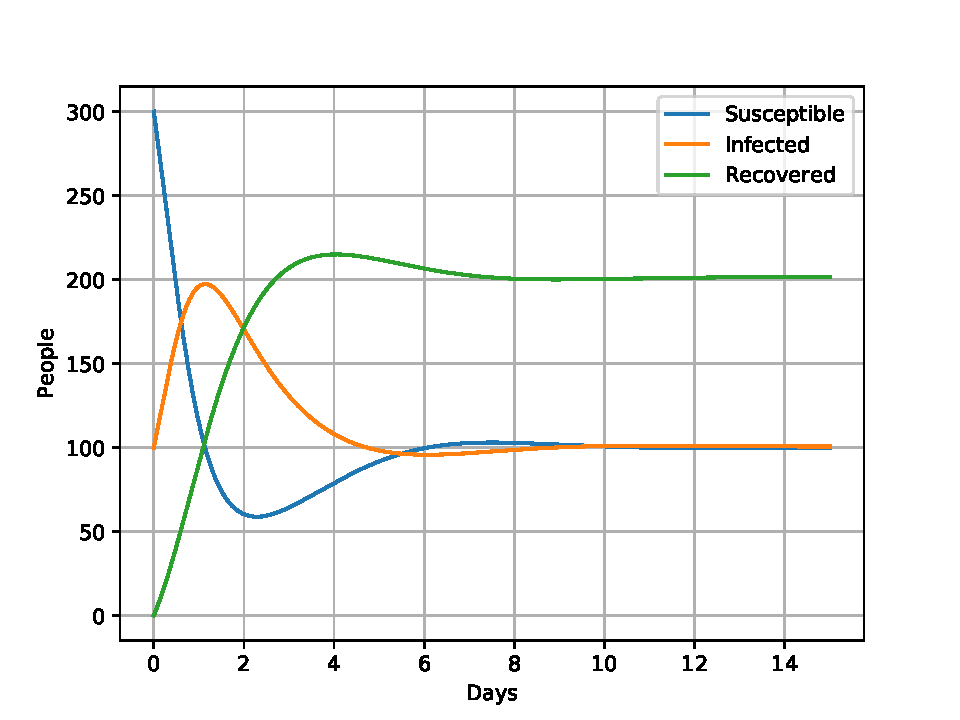
\includegraphics[scale=0.6]{../plots/opp_a_A.pdf}
			\caption{A plot of the population distribution for the SIRS-model using Runge Kutta, for population $A$, where $a=4$, $b=1$ and $c=0.5$. }\label{fig:opp_a_A}
		\end{minipage}
		\begin{minipage}{0.49\textwidth}
			\centering
			\captionsetup{type=table} %% tell latex to change to table
			\begin{tabular}{|l|l|l|l|}
				\hline
				Group & Expected & Numerical   & Number  \\ \hline
				$s^*$ & 0.25 & 0.2499 & 100.0 \\ \hline
				$i^*$ & 0.25 & 0.2516 & 100.6 \\ \hline
				$r^*$ & 0.5  & 0.5035 & 201.4 \\ \hline
			\end{tabular}
			\caption{The corresponding end values for figure \ref{fig:opp_a_A}. The expected values are derived from equation \ref{SIRS_eq}, the numerical values are the potion of the population found by RK4, and number are the total number  of people this corresponds to.}\label{tab:opp_a_A}
		\end{minipage}
		%	\caption{stuff}
	\end{figure}
	
	\begin{figure}[!htb]
		\centering
		\begin{minipage}{0.49\textwidth}
			\centering
			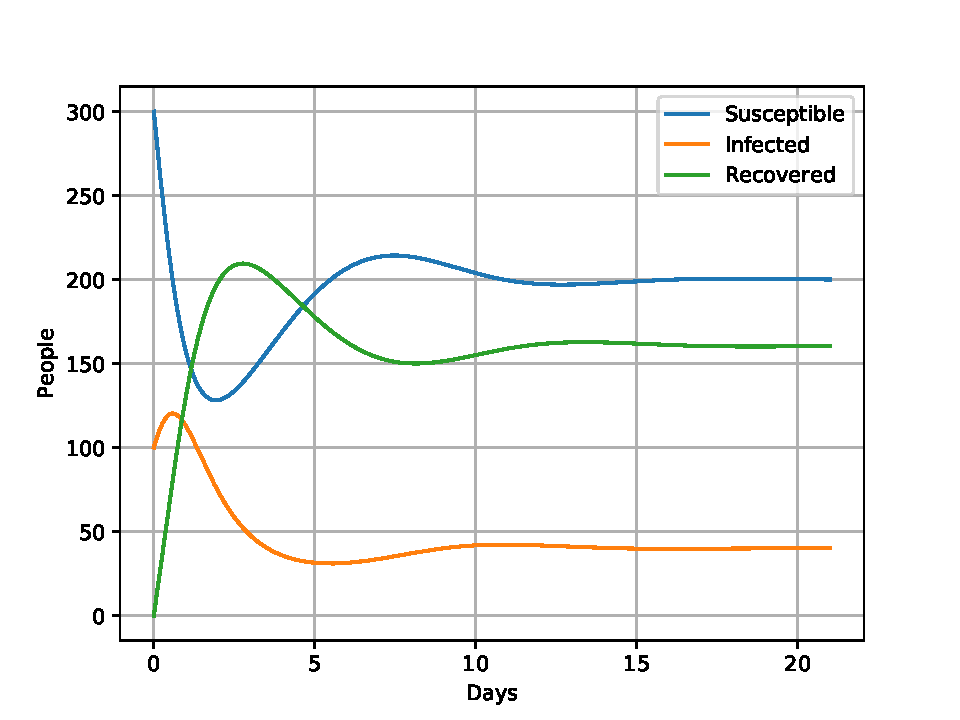
\includegraphics[scale=0.6]{../plots/opp_a_B.pdf}
			\caption{A plot of the population distribution for the SIRS-model using Runge Kutta, for population $B$, where $a=4$, $b=2$ and $c=0.5$. }\label{fig:opp_a_B}
		\end{minipage}
		\begin{minipage}{0.49\textwidth}
			\centering
			\captionsetup{type=table} %% tell latex to change to table
			\begin{tabular}{|l|l|l|l|}
				\hline
				Group & Expected & Numerical   & Number  \\ \hline
				$s^*$ & 0.5 & 0.5001 & 200.1 \\ \hline
				$i^*$ & 0.1 & 0.1006 & 40.2 \\ \hline
				$r^*$ & 0.4 & 0.4011 & 160.5 \\ \hline
			\end{tabular}
			\caption{The corresponding end values for figure \ref{fig:opp_a_B}. The expected values are derived from equation \ref{SIRS_eq}, the numerical values are the potion of the population found by RK4, and number are the total number  of people this corresponds to.}\label{tab:opp_a_B}
		\end{minipage}
		%	\caption{stuff}
	\end{figure}
	
	\begin{figure}[!htb]
		\centering
		\begin{minipage}{0.49\textwidth}
			\centering
			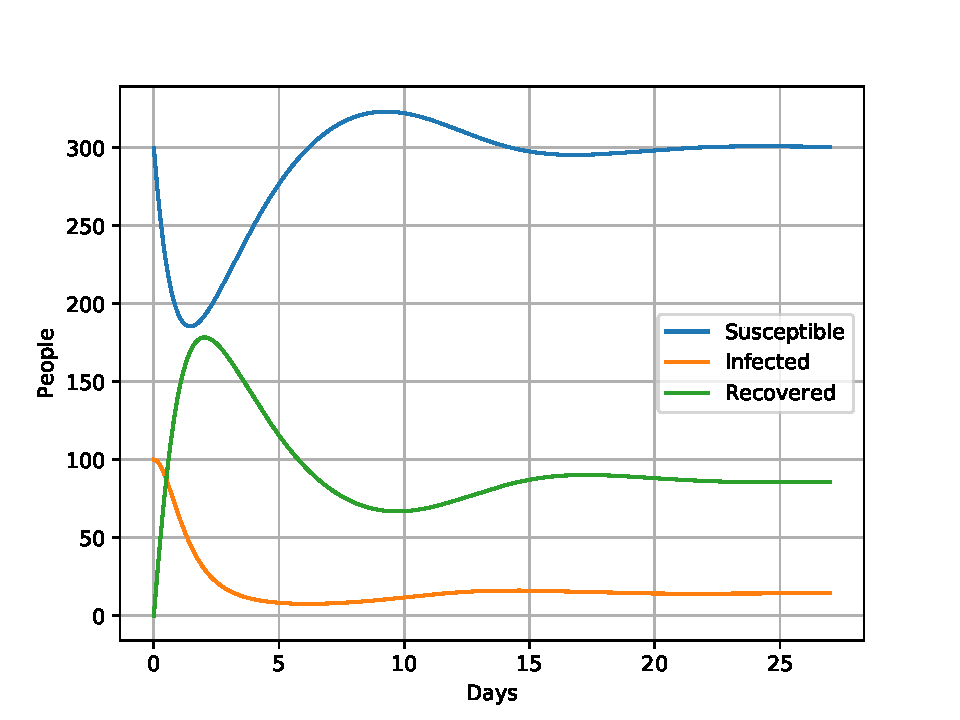
\includegraphics[scale=0.6]{../plots/opp_a_C.pdf}
			\caption{A plot of the population distribution for the SIRS-model using Runge Kutta, for population $C$, where $a=4$, $b=3$ and $c=0.5$. }\label{fig:opp_a_C}
		\end{minipage}
		\begin{minipage}{0.49\textwidth}
			\centering
			\captionsetup{type=table} %% tell latex to change to table
			\begin{tabular}{|l|l|l|l|}
				\hline
				Group & Expected & Numerical   & Number  \\ \hline
				$s^*$ & 0.75 & 0.7511 & 300.5 \\ \hline
				$i^*$ & 0.0357 & 0.0360 & 14.4 \\ \hline
				$r^*$ & 0.2143 & 0.2145 & 85.8 \\ \hline
			\end{tabular}
			\caption{The corresponding end values for figure \ref{fig:opp_a_C}. The expected values are derived from equation \ref{SIRS_eq}, the numerical values are the potion of the population found by RK4, and number are the total number  of people this corresponds to.}\label{tab:opp_a_C}
		\end{minipage}
		%	\caption{stuff}
	\end{figure}
	
	\begin{figure}[!htb]
		\centering
		\begin{minipage}{0.49\textwidth}
			\centering
			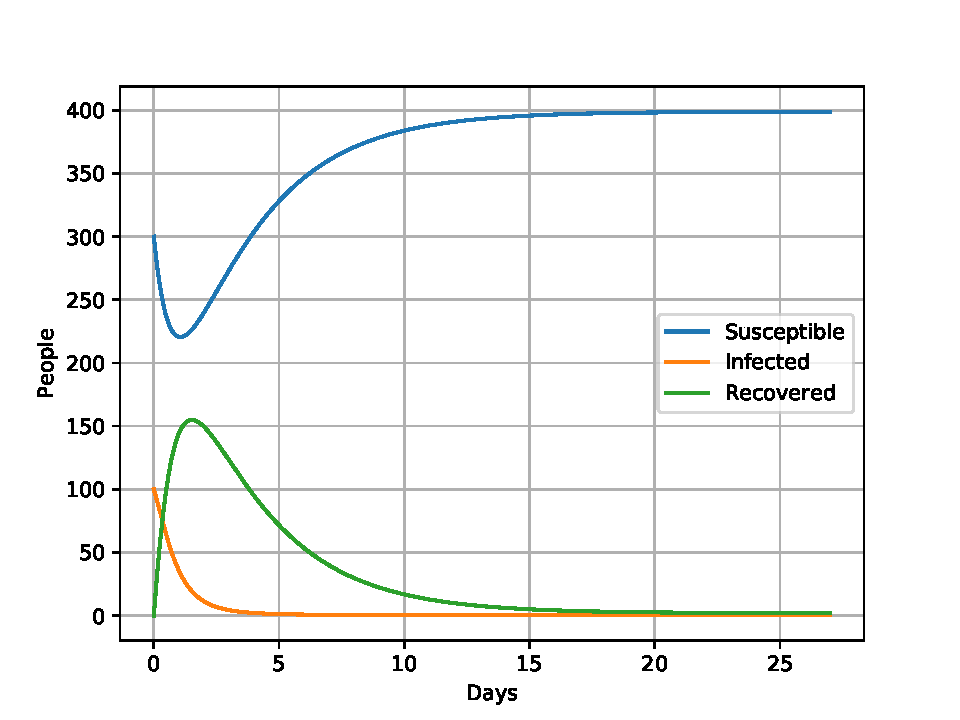
\includegraphics[scale=0.6]{../plots/opp_a_D.pdf}
			\caption{A plot of the population distribution for the SIRS-model using Runge Kutta, for population $D$, where $a=4$, $b=4$ and $c=0.5$. }\label{fig:opp_a_D}
		\end{minipage}
		\begin{minipage}{0.49\textwidth}
			\centering
			\captionsetup{type=table} %% tell latex to change to table
			\begin{tabular}{|l|l|l|l|}
				\hline
				Group & Expected & Numerical   & Number  \\ \hline
				$s^*$ & 1.0 & 0.9974 & 399.0 \\ \hline
				$i^*$ & 0.0 & 0.0006 & 0.2 \\ \hline
				$r^*$ & 0.0 & 0.0047 & 1.9 \\ \hline
			\end{tabular}
			\caption{The corresponding end values for figure \ref{fig:opp_a_D}. The expected values are derived from equation \ref{SIRS_eq}, the numerical values are the potion of the population found by RK4, and number are the total number  of people this corresponds to.}\label{tab:opp_a_D}
		\end{minipage}
		%	\caption{stuff}
	\end{figure}
	
	\begin{figure}[!htb]
		\centering
		\begin{minipage}{0.49\textwidth}
			\centering
			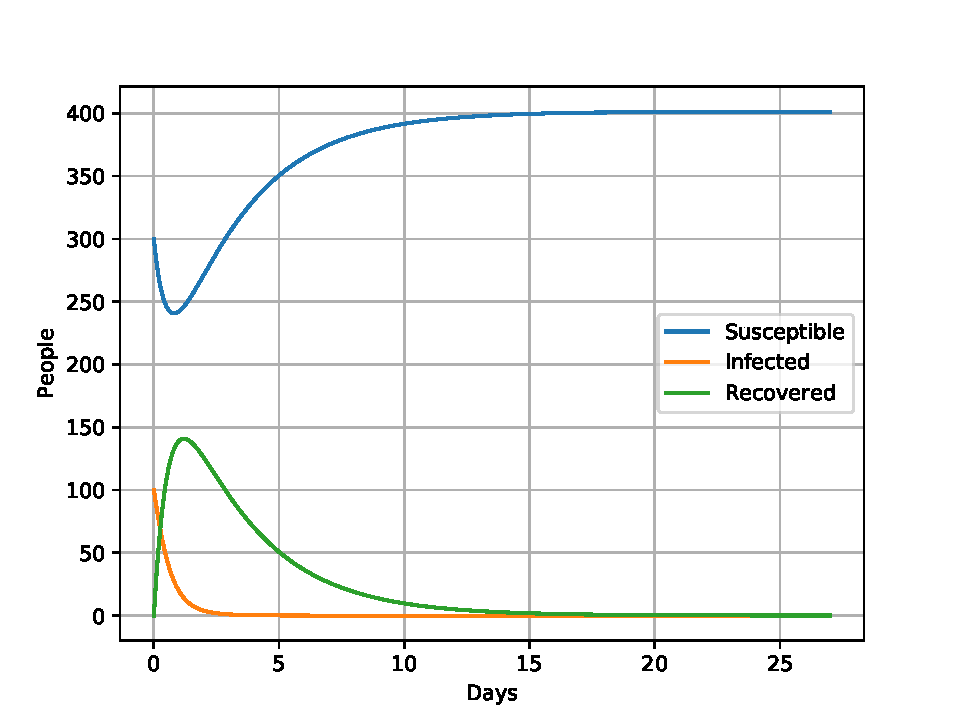
\includegraphics[scale=0.6]{../plots/opp_a_E.pdf}
			\caption{A plot of the population distribution for the SIRS-model using Runge Kutta, for population $E$, where $a=4$, $b=5$ and $c=0.5$. }\label{fig:opp_a_E}
		\end{minipage}
		\begin{minipage}{0.49\textwidth}
			\centering
			\captionsetup{type=table} %% tell latex to change to table
			\begin{tabular}{|l|l|l|l|}
				\hline
				Group & Expected & Numerical   & Number  \\ \hline
				$s^*$ & 1.25 & 1.0034 & 401.4 \\ \hline
				$i^*$ & -0.0227 & $4.7119\cdot 10^{-11}$ & $1.9\cdot 10^{-8}$ \\ \hline
				$r^*$ & -0.2273 & $8.4064\cdot 10^{-5}$ & $3.4\cdot 10^{-2}$ \\ \hline
			\end{tabular}
			\caption{The corresponding end values for figure \ref{fig:opp_a_E}. The expected values are derived from equation \ref{SIRS_eq}, the numerical values are the potion of the population found by RK4, and number are the total number  of people this corresponds to.}\label{tab:opp_a_E}
		\end{minipage}
		%	\caption{stuff}
	\end{figure}
	
	
	\subsection{Monte Carlo}
	\begin{figure}[!htb]
		\centering
		\begin{minipage}{0.49\textwidth}
			\centering
			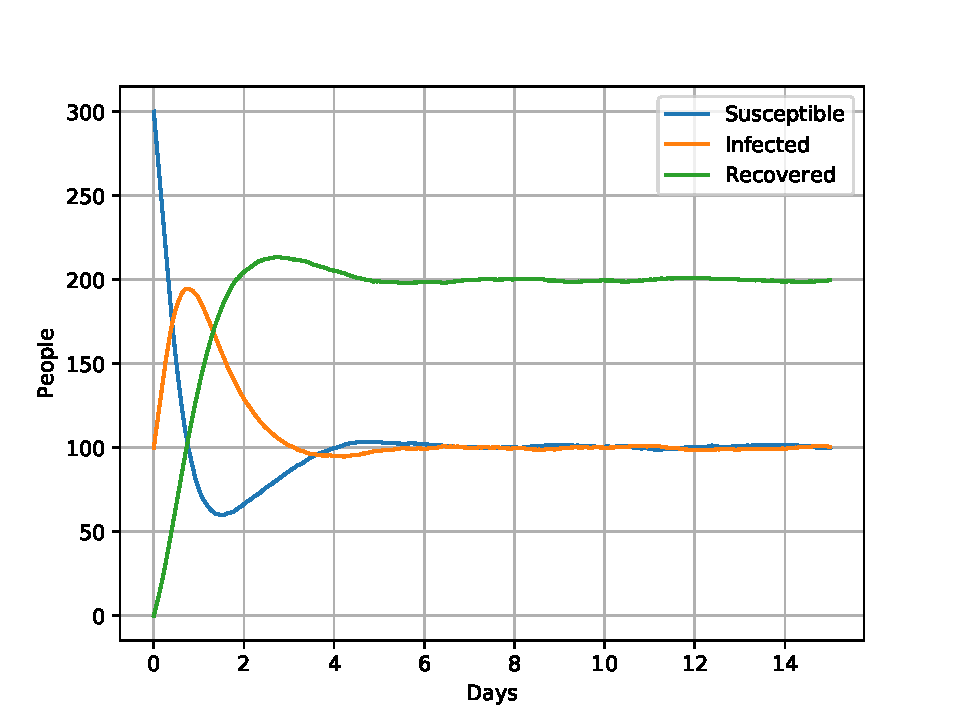
\includegraphics[scale=0.6]{../plots/opp_a_A_MC.pdf}
			\caption{A plot of the population distribution for the SIRS-model using Monte Carlo, for population $A$, where $a=4$, $b=1$ and $c=0.5$. }\label{fig:opp_a_A_MC}
		\end{minipage}
		\begin{minipage}{0.49\textwidth}
			\centering
			\captionsetup{type=table} %% tell latex to change to table
			\begin{tabular}{|l|l|l|l|l|}
				\hline
				Group & Expected & Numerical   & Number  & $\sigma$\\ \hline
				$s^*$ & 0.25 & 0.2499 & 99.98 & 11.88\\ \hline
				$i^*$ & 0.25 & 0.2511 & 100.43 & 10.33\\ \hline
				$r^*$ & 0.5  & 0.4989 & 199.60 & 8.84\\ \hline
			\end{tabular}
			\caption{The corresponding end values and standard deviations for figure \ref{fig:opp_a_A_MC}. The expected values are derived from equation \ref{SIRS_eq}, the numerical values are the portion of the population found by the Monte Carlo simulation, and number is the total number of people this corresponds to.}\label{tab:opp_a_A_mc}
		\end{minipage}
		%	\caption{stuff}
	\end{figure}
	
	\begin{figure}[!htb]
		\centering
		\begin{minipage}{0.49\textwidth}
			\centering
			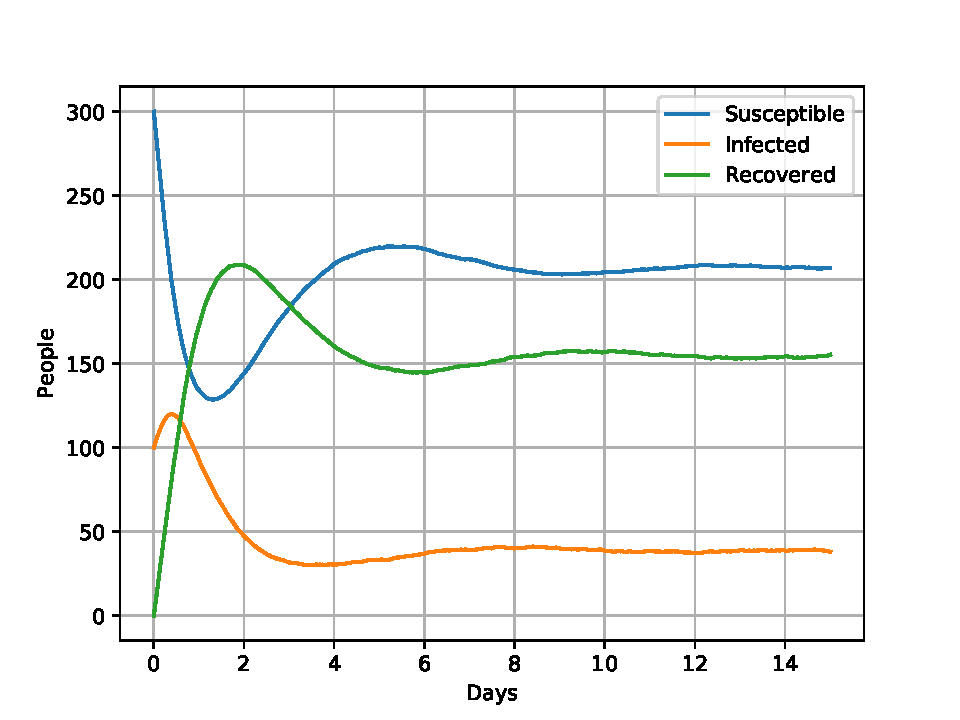
\includegraphics[scale=0.6]{../plots/opp_a_B_MC.pdf}
			\caption{A plot of the population distribution for the SIRS-model using Monte Carlo, for population $B$, where $a=4$, $b=2$ and $c=0.5$. }\label{fig:opp_a_B_MC}
		\end{minipage}
		\begin{minipage}{0.49\textwidth}
			\centering
			\captionsetup{type=table} %% tell latex to change to table
			\begin{tabular}{|l|l|l|l|l|}
				\hline
				Group & Expected & Numerical   & Number  & $\sigma$\\ \hline
				$s^*$ & 0.5 & 0.5171 & 206.85 & 31.13\\ \hline
				$i^*$ & 0.1 & 0.0949 & 37.94 & 11.79\\ \hline
				$r^*$ & 0.4 & 0.3880 & 155.21 & 24.56\\ \hline
			\end{tabular}
			\caption{The corresponding end values and standard deviations for figure \ref{fig:opp_a_B_MC}. The expected values are derived from equation \ref{SIRS_eq}, the numerical values are the portion of the population found by the Monte Carlo simulation, and number is the total number of people this corresponds to.}\label{tab:opp_a_B_mc}
		\end{minipage}
		%	\caption{stuff}
	\end{figure}
	
	\begin{figure}[!htb]
		\centering
		\begin{minipage}{0.49\textwidth}
			\centering
			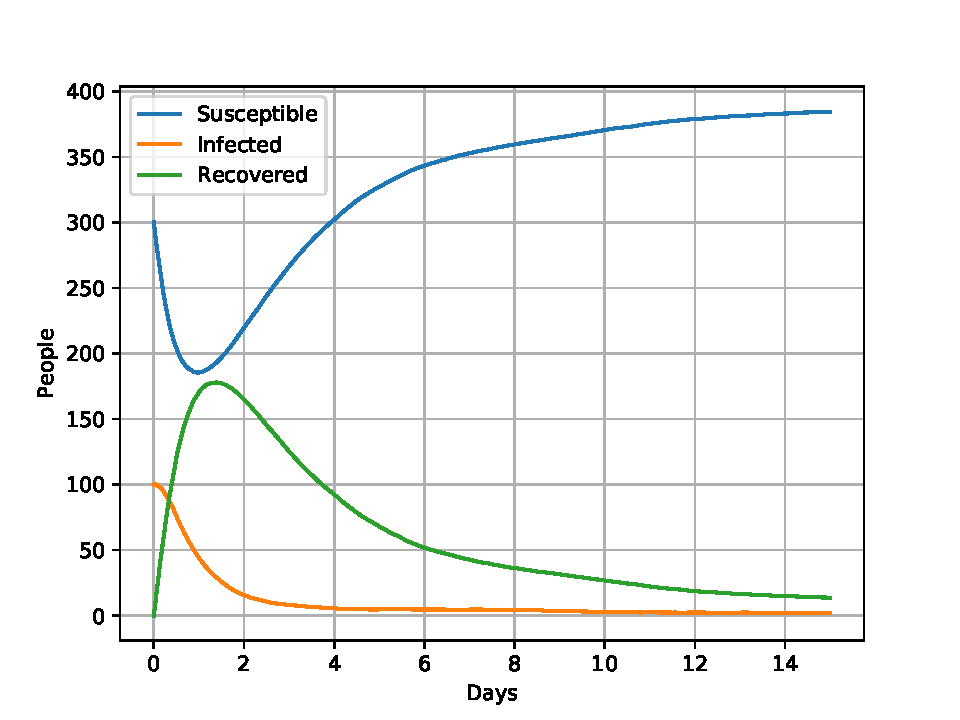
\includegraphics[scale=0.6]{../plots/opp_a_C_MC.pdf}
			\caption{A plot of the population distribution for the SIRS-model using Monte Carlo, for population $C$, where $a=4$, $b=3$ and $c=0.5$. }\label{fig:opp_a_C_MC}
		\end{minipage}
		\begin{minipage}{0.49\textwidth}
			\centering
			\captionsetup{type=table} %% tell latex to change to table
			\begin{tabular}{|l|l|l|l|l|}
				\hline
				Group & Expected & Numerical   & Number  & $\sigma$\\ \hline
				$s^*$ & 0.75 & 0.9614 & 384.55 & 34.83\\ \hline
				$i^*$ & 0.04 & 0.0045 & 1.78 & 5.31\\ \hline
				$r^*$ & 0.21 & 0.0342 & 13.67 & 30.25\\ \hline
			\end{tabular}
			\caption{The corresponding end values and standard deviations for figure \ref{fig:opp_a_C_MC}. The expected values are derived from equation \ref{SIRS_eq}, the numerical values are the portion of the population found by the Monte Carlo simulation, and number is the total number of people this corresponds to.}\label{tab:opp_a_C_mc}
		\end{minipage}
		%	\caption{stuff}
	\end{figure}
	
	\begin{figure}[!htb]
		\centering
		\begin{minipage}{0.49\textwidth}
			\centering
			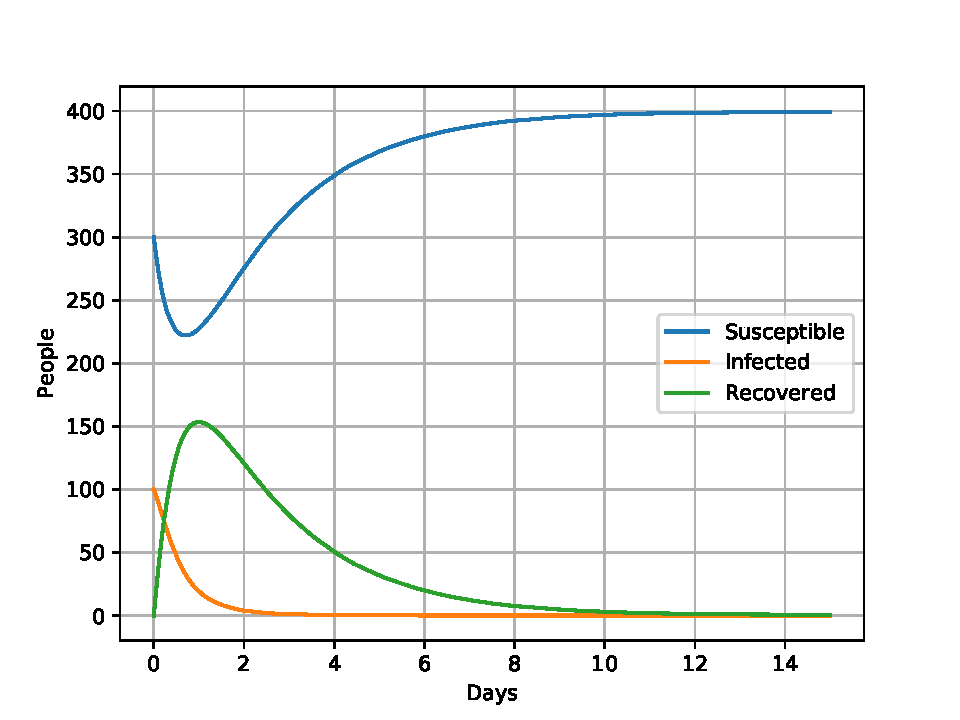
\includegraphics[scale=0.6]{../plots/opp_a_D_MC.pdf}
			\caption{A plot of the population distribution for the SIRS-model using Monte Carlo, for population $D$, where $a=4$, $b=4$ and $c=0.5$. }\label{fig:opp_a_D_MC}
		\end{minipage}
		\begin{minipage}{0.49\textwidth}
			\centering
			\captionsetup{type=table} %% tell latex to change to table
			\begin{tabular}{|l|l|l|l|l|}
				\hline
				Group & Expected & Numerical   & Number  & $\sigma$\\ \hline
				$s^*$ & 1.0 & 0.9989 & 399.55 & 3.19\\ \hline
				$i^*$ & 0.0 & 0.0 & 0.0 & 0.0\\ \hline
				$r^*$ & 0.0 & 0.0011 & 0.45 & 3.19\\ \hline
			\end{tabular}
			\caption{The corresponding end values and standard deviations for figure \ref{fig:opp_a_D_MC}. The expected values are derived from equation \ref{SIRS_eq}, the numerical values are the portion of the population found by the Monte Carlo simulation, and number is the total number of people this corresponds to.}\label{tab:opp_a_D_mc}
		\end{minipage}
		%	\caption{stuff}
	\end{figure}
	
	\begin{figure}[!htb]
		\centering
		\begin{minipage}{0.49\textwidth}
			\centering
			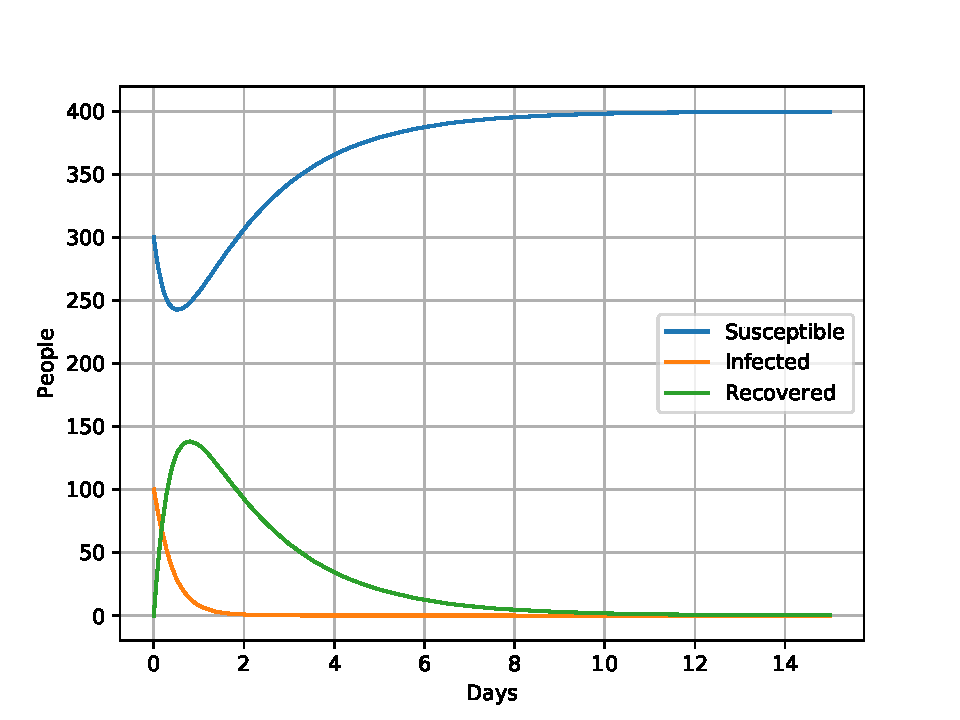
\includegraphics[scale=0.6]{../plots/opp_a_E_MC.pdf}
			\caption{A plot of the population distribution for the SIRS-model using Monte Carlo, for population $E$, where $a=4$, $b=5$ and $c=0.5$. }\label{fig:opp_a_E_MC}
		\end{minipage}
		\begin{minipage}{0.49\textwidth}
			\centering
			\captionsetup{type=table} %% tell latex to change to table
			\begin{tabular}{|l|l|l|l|l|}
				\hline
				Group & Expected & Numerical   & Number  & $\sigma$\\ \hline
				$s^*$ & 1.25 & 0.9996 & 399.84 & 0.40\\ \hline
				$i^*$ & -0.023 & 0.0 & 0.0 & 0.0\\ \hline
				$r^*$ & -0.023 & 0.0004 & 0.16 & 0.40\\ \hline
			\end{tabular}
			\caption{The corresponding end values and standard deviations for figure \ref{fig:opp_a_E_MC}. The expected values are derived from equation \ref{SIRS_eq}, and clearly break down for this population, the numerical values are the portion of the population found by the Monte Carlo simulation, and number is the total number of people this corresponds to.}\label{tab:opp_a_E_mc}
		\end{minipage}
		%	\caption{stuff}
	\end{figure}
	
	
	\subsection{Improving the model}
	
	\subsubsection{Vital dynamics}
	
	Plots of population $B$ when accounting for vital dynamics, found using Runge Kutta, can be seen in figure \ref{opp_c0B}. In figure \ref{opp_c0} you can see plots of population $A$ where $d_i$ either too high or low to realistically kill the entire population, while in figure \ref{opp_c1} you can see a plot where $d_i$ is the correct size to kill the entire population. Finally, in figure \ref{opp_c2} you can see a plot where $d$ and $e$ have been increased by a factor of 1000000. 
	
	\begin{figure}[!htb]
		\centering 
		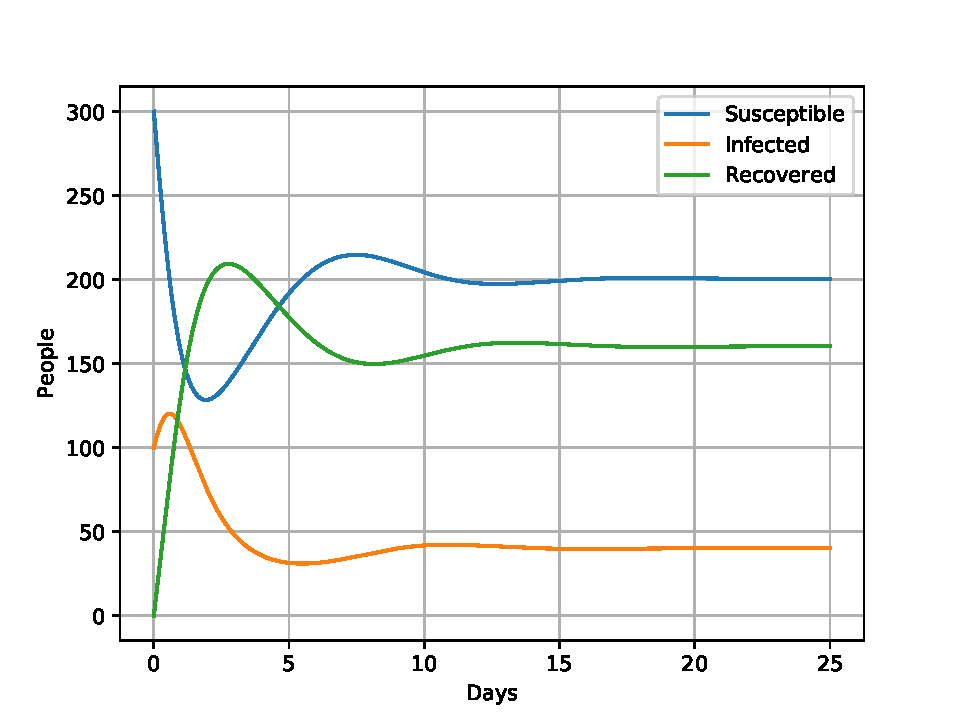
\includegraphics[scale=0.56]{../plots/opp_c_B0.pdf}
		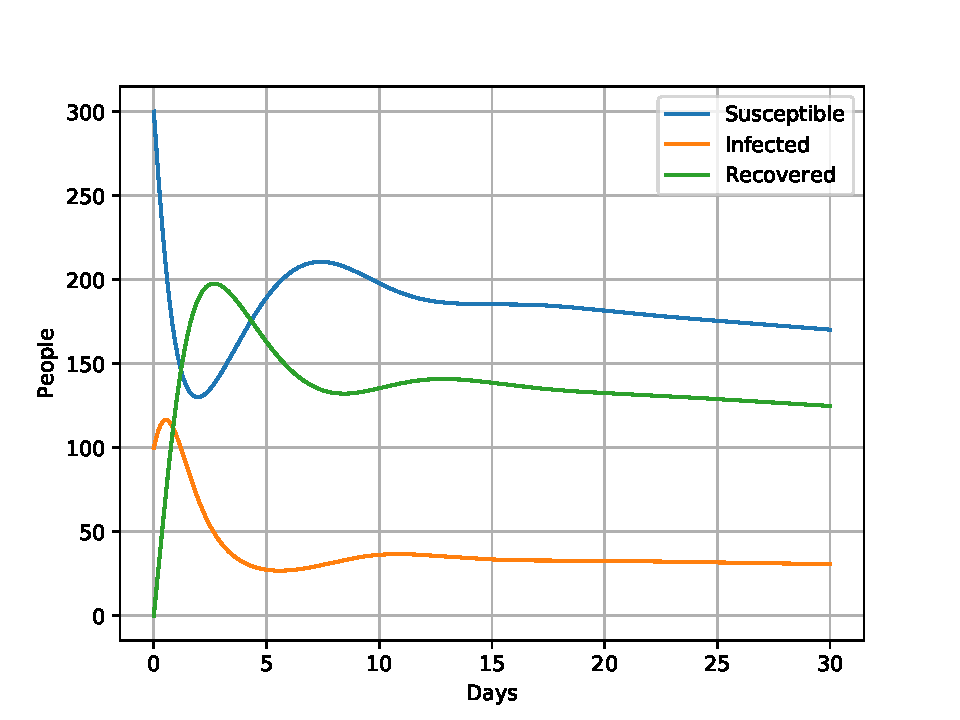
\includegraphics[scale=0.56]{../plots/opp_c_B1.pdf}
		\caption{Plots of population $B$ when accounting for vital dynamics, found using Runge Kutta. On the left $d_i=0$ and on the rigth $d_i=0.1$.}
		%Label gjør det enkelt å referere til ulike bilder.
		\label{opp_c0B}
	\end{figure}
	
	\begin{figure}[!htb]
		\centering 
		%Scale angir størrelsen på bildet. Bildefilen må ligge i samme mappe som tex-filen. 
		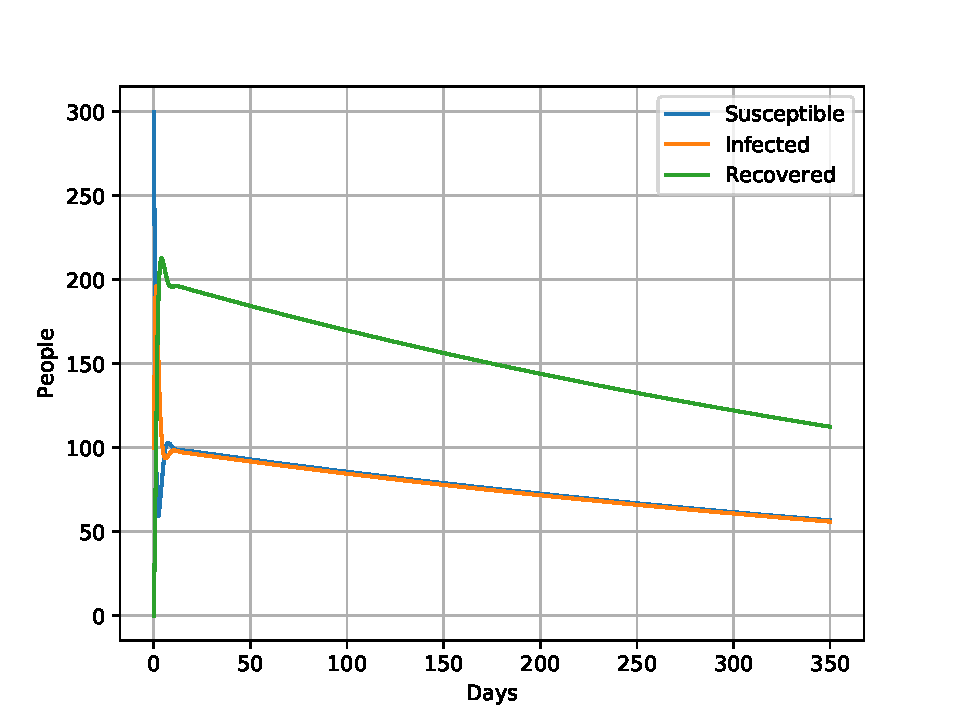
\includegraphics[scale=0.56]{../plots/opp_c_k3.pdf} %kan kaskje være først?
		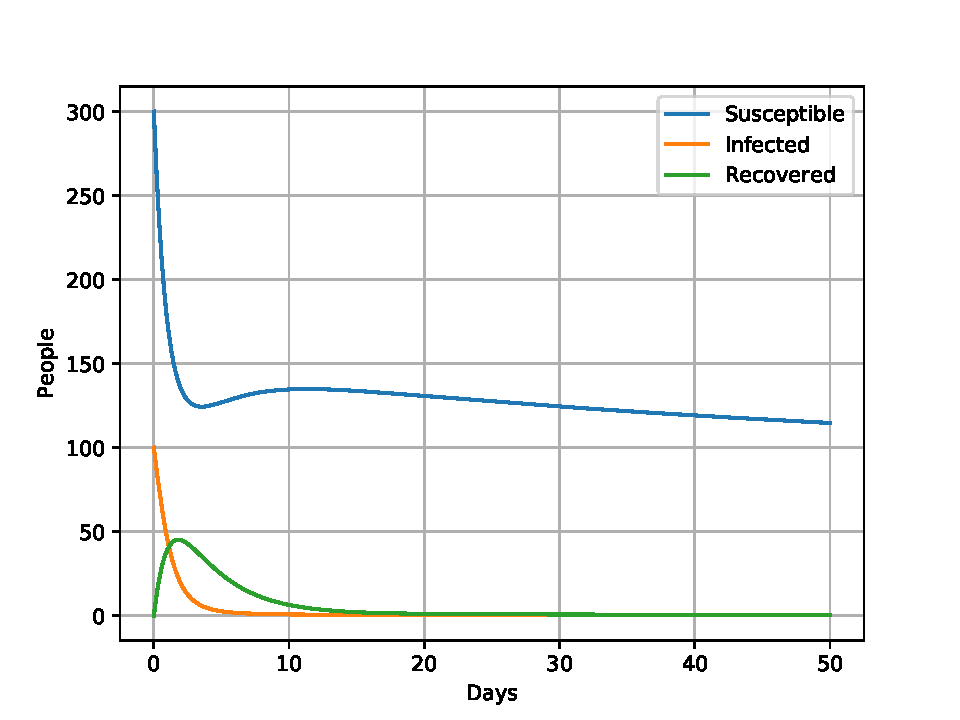
\includegraphics[scale=0.56]{../plots/opp_c_k0.pdf}
		\caption{Plots of population $A$ when accounting for vital dynamics, found using Runge Kutta. On the left $d_i=0.01$ and on the rigth $d_i=3$. The left $d_i$ is too low to effectively kill the entire population, while the one is too large.}
		\label{opp_c0}
	\end{figure}

	\begin{figure}[!htb]
		\centering 
		%	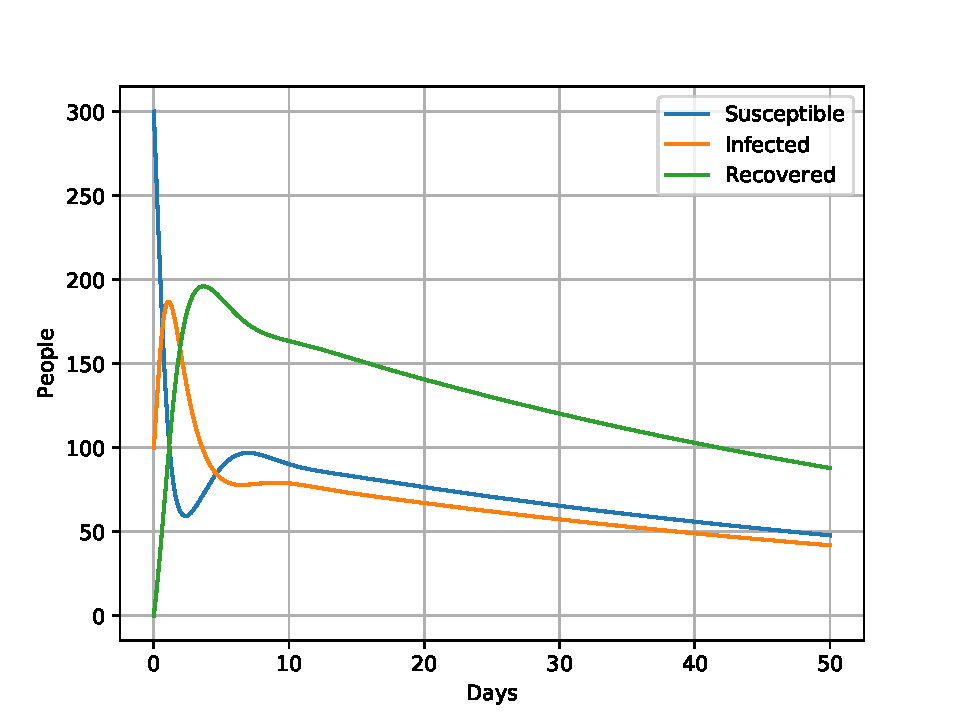
\includegraphics[scale=0.56]{../plots/opp_c_k2.pdf}
		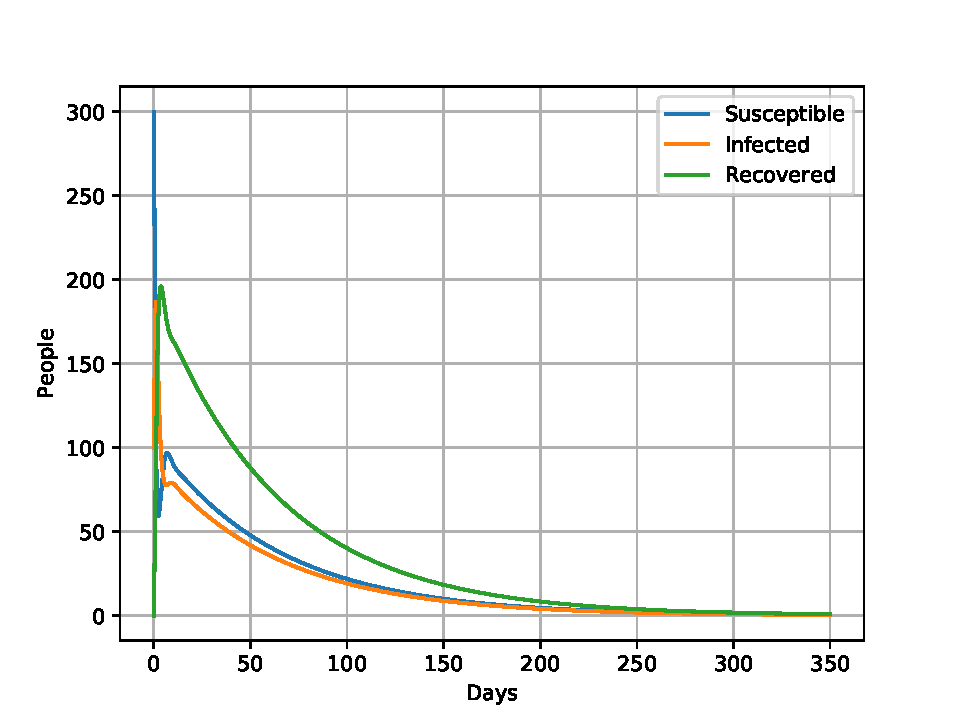
\includegraphics[scale=0.56]{../plots/opp_c_k2l.pdf}	
		%mulig jeg bør splitte denne
		\caption{Plots of population $A$ when accounting for vital dynamics, found using Runge Kutta, with $d_i=0.1$. Here $d_i$ is the correct size to kill the entire population. }
		%Label gjør det enkelt å referere til ulike bilder.
		\label{opp_c1}
	\end{figure}
	
	\begin{figure}[!htb]
		\centering 
		%Scale angir størrelsen på bildet. Bildefilen må ligge i samme mappe som tex-filen. 	
		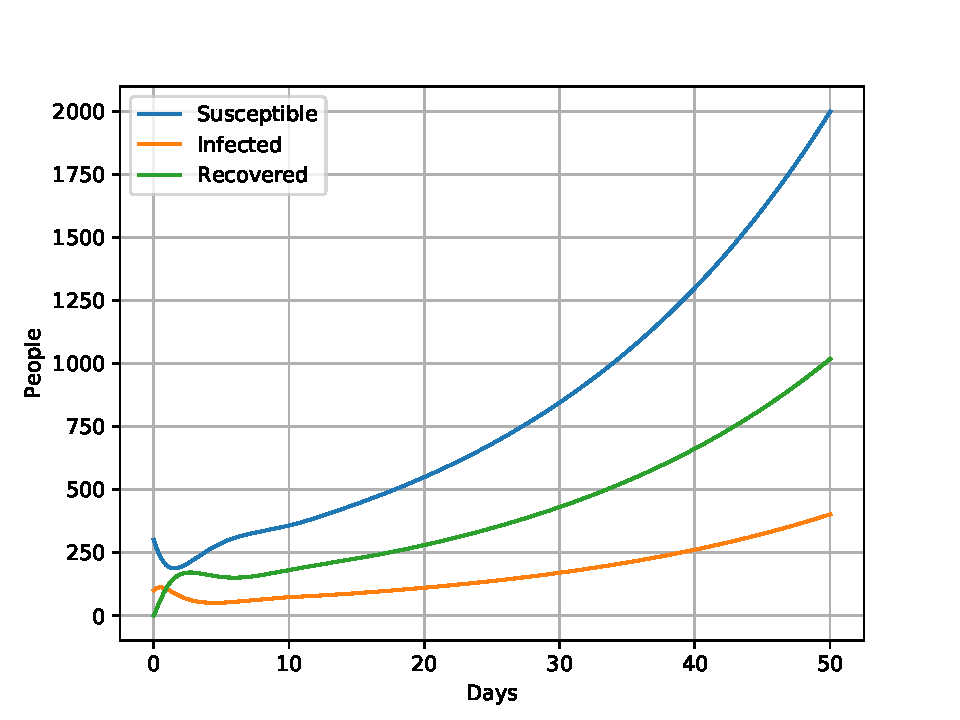
\includegraphics[scale=0.56]{../plots/opp_c_h_100000.pdf} %denne?
		\caption{Plots of population $B$  when accounting for vital dynamics, found using Runge Kutta, with $d_i=0.1$, and $d$ and $e$ are increased by a factor of 
			%	1000, 2000 and 
			1000000 
			.}
		%Label gjør det enkelt å referere til ulike bilder.
		\label{opp_c2}
	\end{figure}
	
	
	
	
		Plots of population $B$ when accounting for vital dynamics, found using Monte Carlo, can be seen in figure \ref{opp_c0B_MC}. In figure \ref{opp_c0_MC} you can see plots of population $A$ where $d_i$ either too high or low to realistically kill the entire population, while in figure \ref{opp_c1_MC} you can see a plot where $d_i$ is the correct size to in some cases kill the entire population, but definitely reduce its size significantly. Finally, in figure \ref{opp_c2_MC} you can see a plot where $d$ and $e$ have been increased by a factor of 1000000. 
	
	\begin{figure}[!htb]
		\centering 
		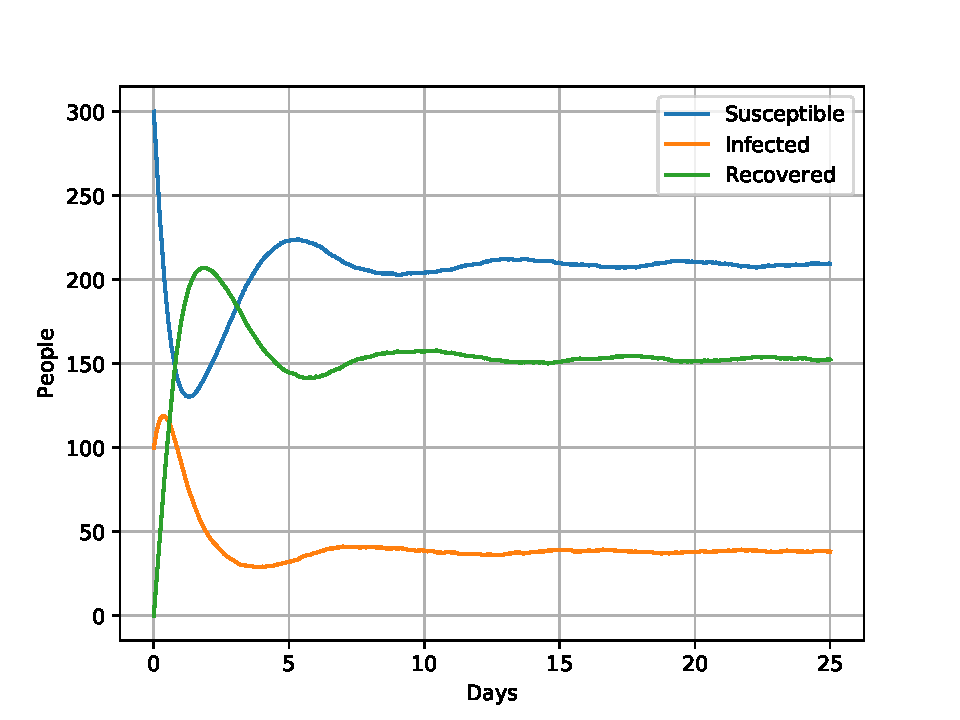
\includegraphics[scale=0.56]{../plots/opp_c_B0_MC.pdf}
		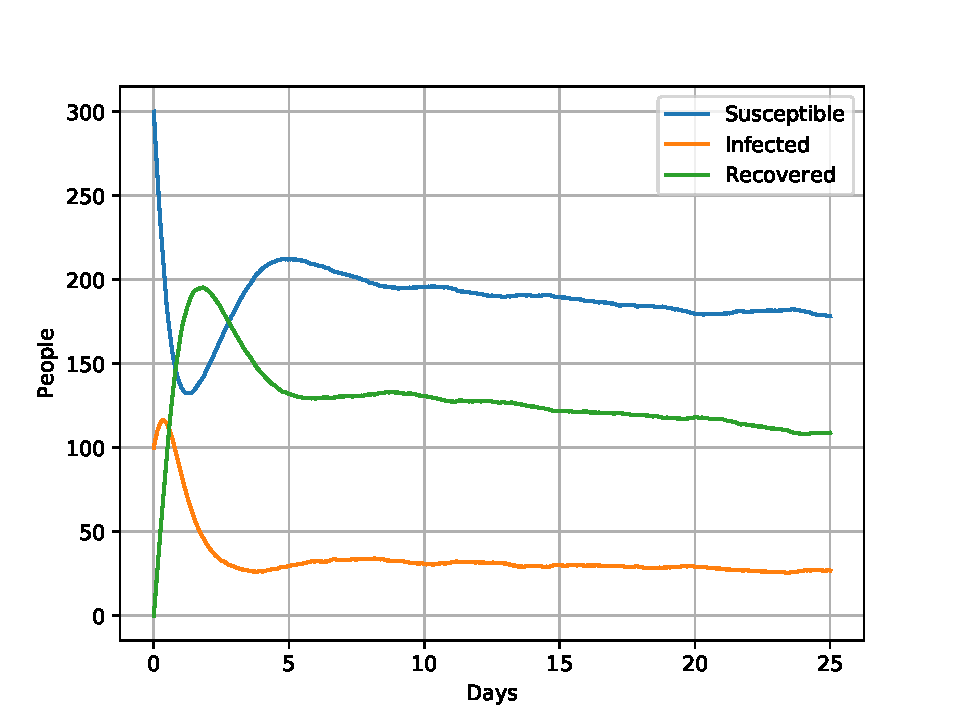
\includegraphics[scale=0.56]{../plots/opp_c_B1_MC.pdf}
		\caption{Plots of population $B$ when accounting for vital dynamics, found using Monte Carlo. On the left $d_i=0$ and on the rigth $d_i=0.1$.}
		%Label gjør det enkelt å referere til ulike bilder.
		\label{opp_c0B_MC}
	\end{figure}
	
	\begin{figure}[!htb]
		\centering 
		%Scale angir størrelsen på bildet. Bildefilen må ligge i samme mappe som tex-filen. 
		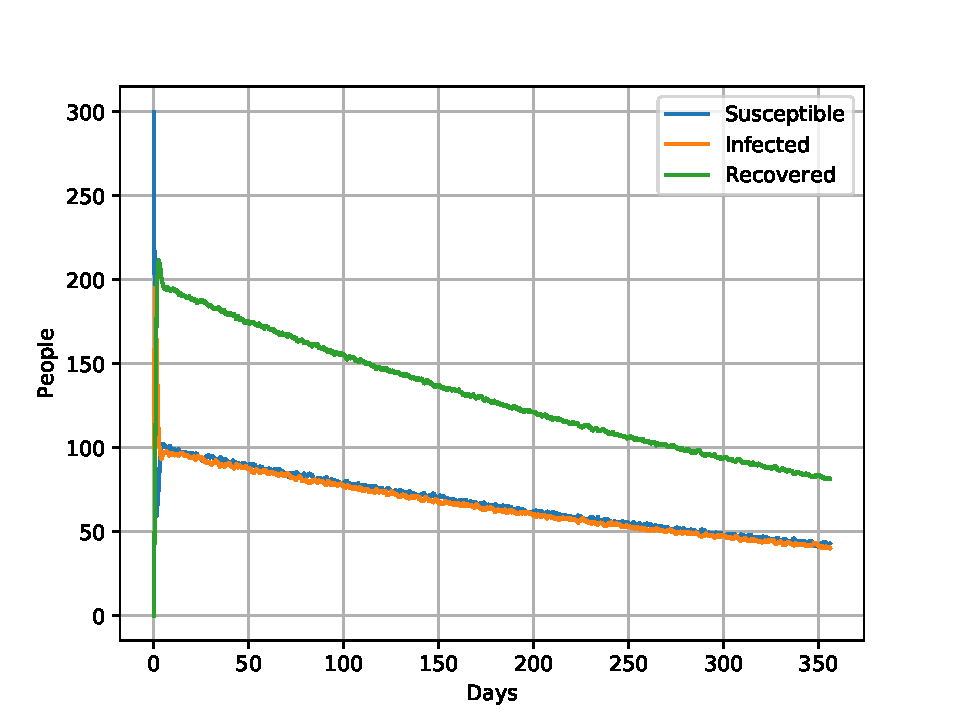
\includegraphics[scale=0.56]{../plots/opp_c_k3_MC.pdf} %kan kaskje være først?
		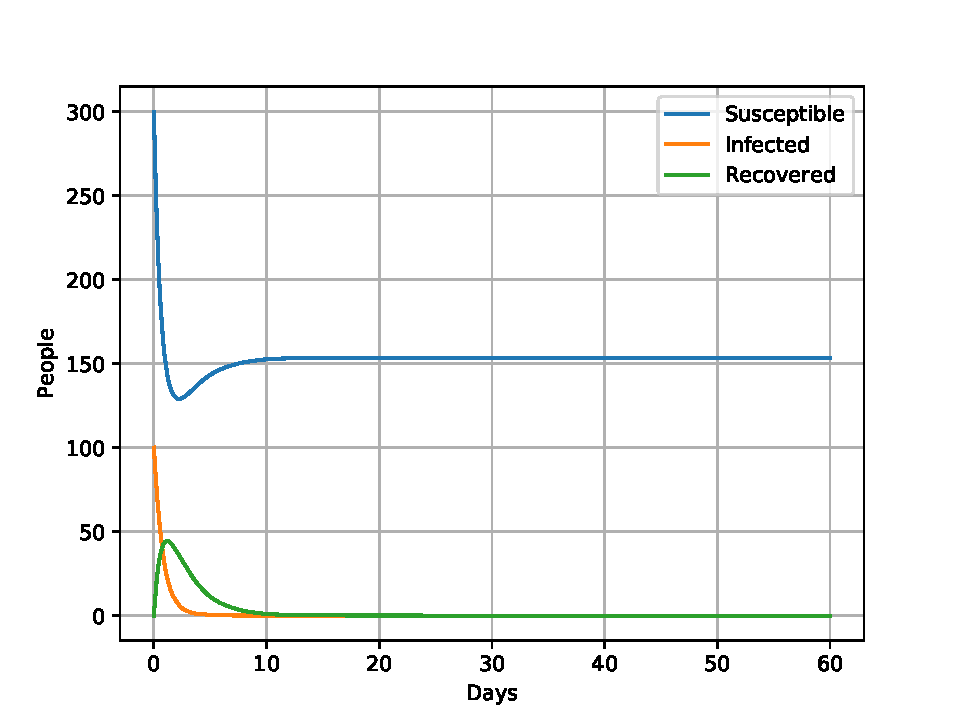
\includegraphics[scale=0.56]{../plots/opp_c_k0_MC.pdf}
		\caption{Plots of population $A$ when accounting for vital dynamics, found using Monte Carlo. On the left $d_i=0.01$ and on the rigth $d_i=3$. The left $d_i$ is too low to effectively kill the entire population, while other the one is too large.}
		\label{opp_c0_MC}
	\end{figure}
	
	\begin{figure}[!htb]
		\centering 
		%	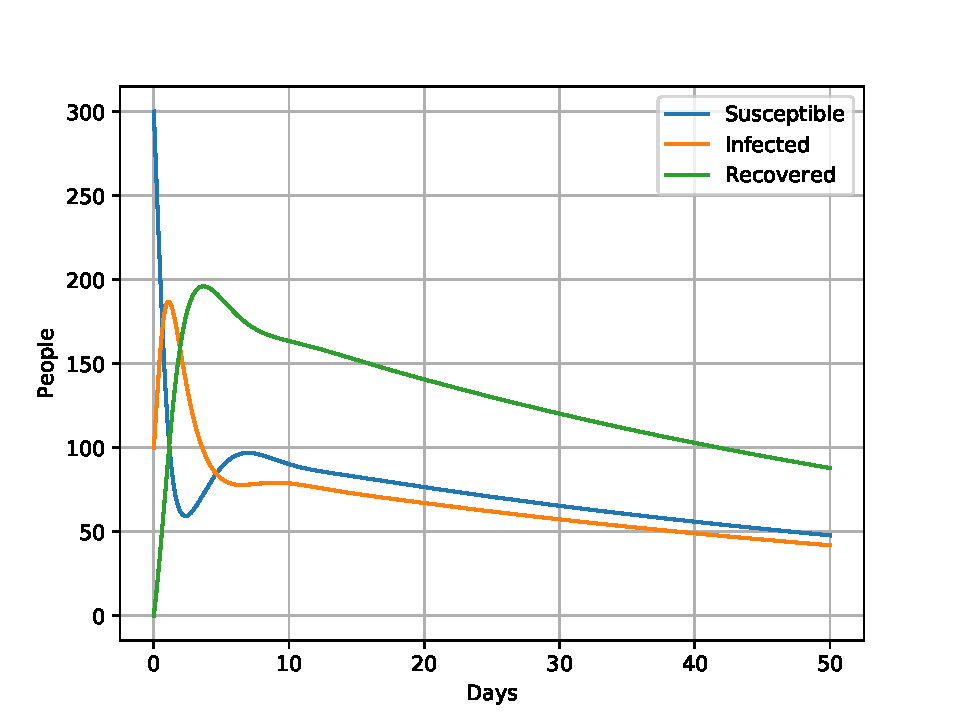
\includegraphics[scale=0.56]{../plots/opp_c_k2.pdf}
		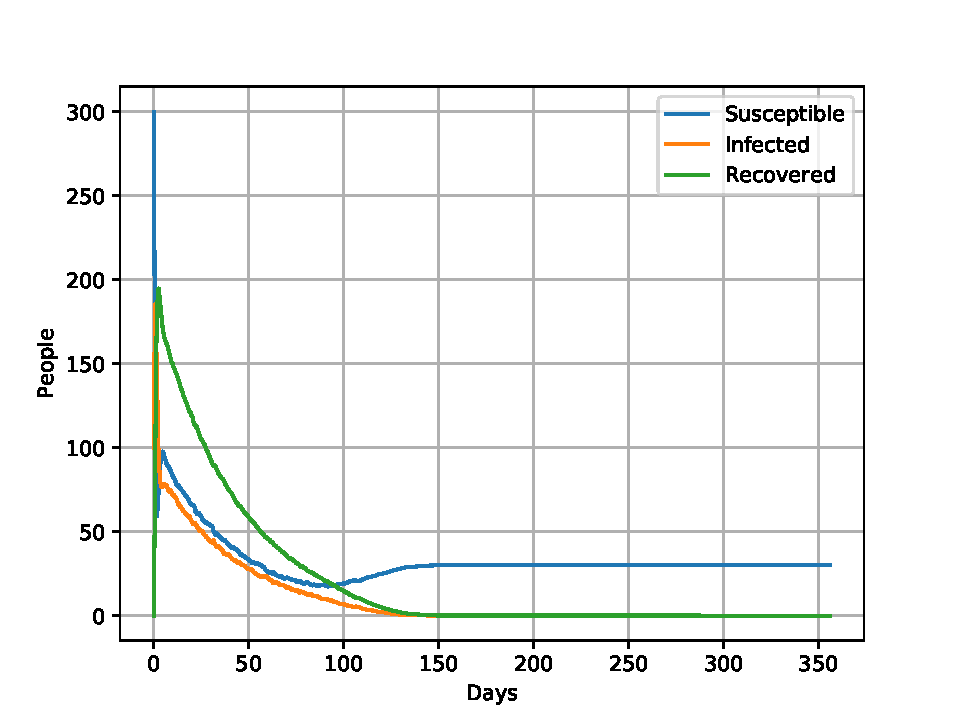
\includegraphics[scale=0.56]{../plots/opp_c_k2l_MC.pdf}	
		%mulig jeg bør splitte denne
		\caption{Plots of population $A$ when accounting for vital dynamics, found using Monte Carlo, with $d_i=0.1$. Here $d_i$ is the correct size to kill most of the population. }
		%Label gjør det enkelt å referere til ulike bilder.
		\label{opp_c1_MC}
	\end{figure}
	
	\begin{figure}[!htb]
		\centering 
		%Scale angir størrelsen på bildet. Bildefilen må ligge i samme mappe som tex-filen. 	
		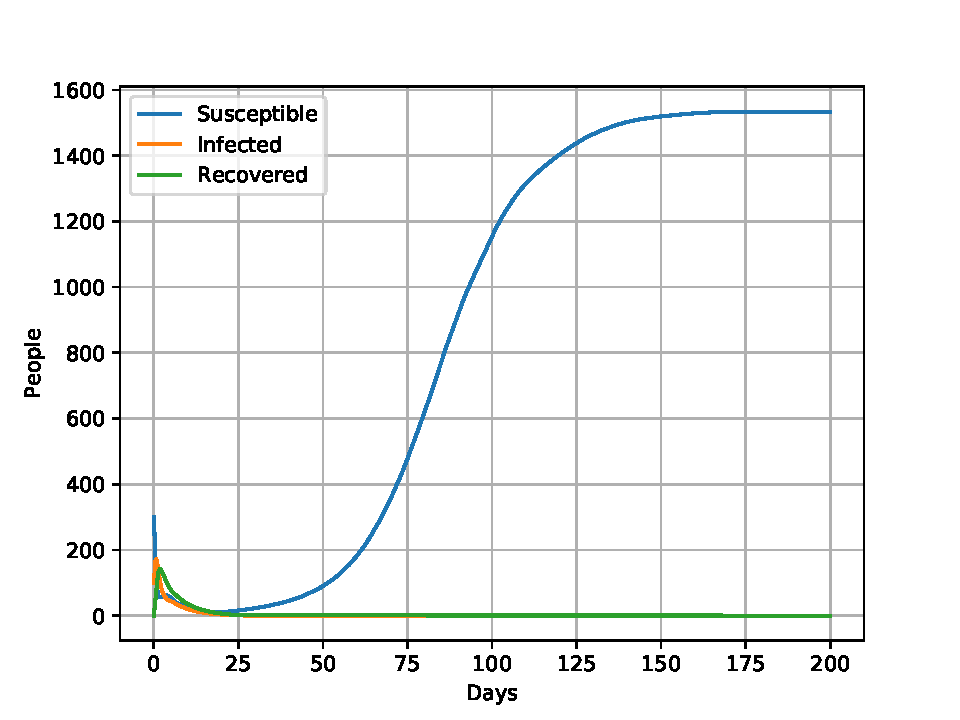
\includegraphics[scale=0.56]{../plots/opp_c_h_1000000_MC.pdf} %denne?
		\caption{Plots of population $B$  when accounting for vital dynamics, found using Monte Carlo, with $d_i=0.1$, and $d$ and $e$ are increased by a factor of 
			%	1000, 2000 and 
			1000000 
			.}
		%Label gjør det enkelt å referere til ulike bilder.
		\label{opp_c2_MC}
	\end{figure}
	
	
	
	\subsubsection{Seasonal Variation}
	
	In figure \ref{opp_d0} you can see a plot of population $A$ and $C$ where $a$ varies with time. 
	
	\begin{figure}[!htb]
		\centering 
		%Scale angir størrelsen på bildet. Bildefilen må ligge i samme mappe som tex-filen. 
		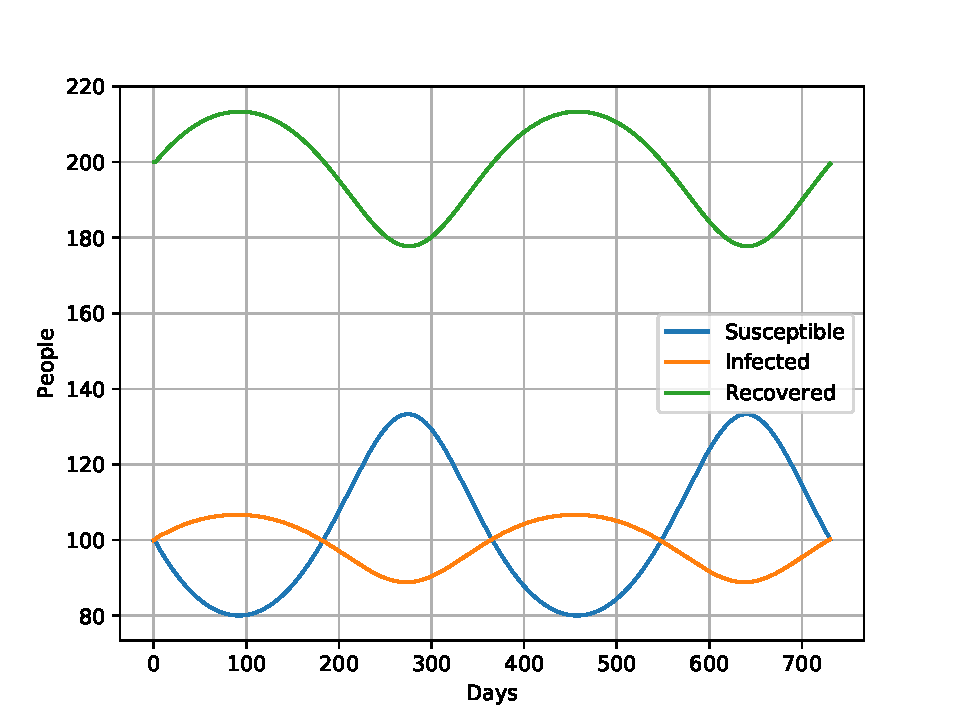
\includegraphics[scale=0.56]{../plots/opp_d_A.pdf}
		%	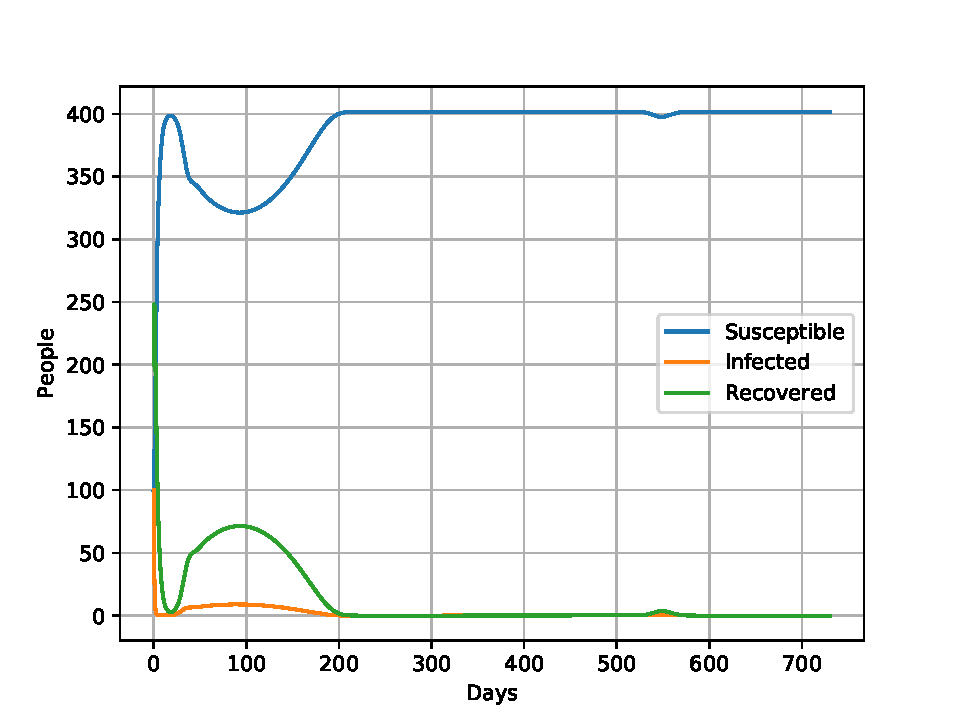
\includegraphics[scale=0.56]{../plots/opp_d_B.pdf}
		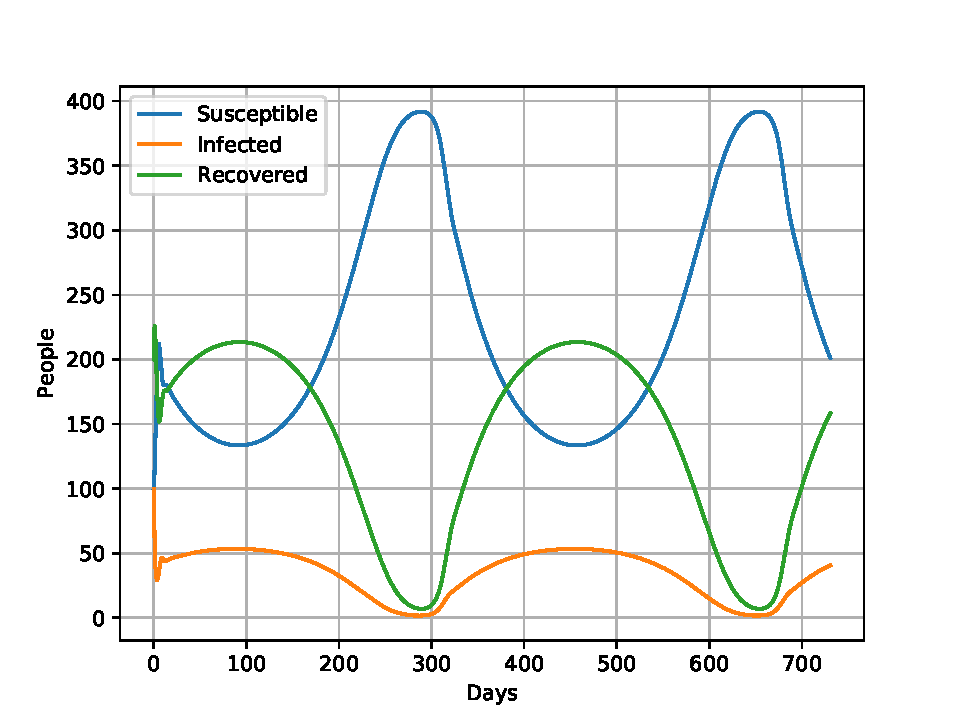
\includegraphics[scale=0.56]{../plots/opp_d_C.pdf}
		\caption{Plots of populations when $a$ varies with time, found using Runge Kutta. Population $A$ on the left with $A=1$ and $a0=4$, and $B$ on the right with $A=2$ and $a0=4$.}
		%Label gjør det enkelt å referere til ulike bilder.
		\label{opp_d0}
	\end{figure}

	In figure \ref{opp_d0_MC} you can see a plot of population $A$ and $C$ where $a$ varies with time. 

	\begin{figure}[!htb]
		\centering 
		%Scale angir størrelsen på bildet. Bildefilen må ligge i samme mappe som tex-filen. 
		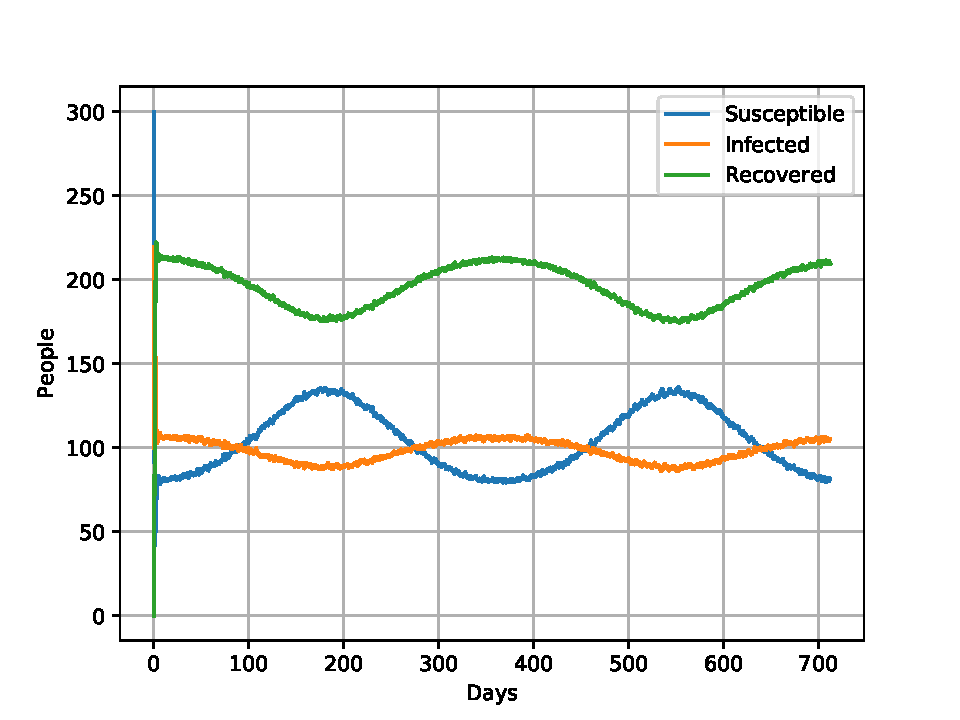
\includegraphics[scale=0.56]{../plots/opp_d_A_MC.pdf}
		%	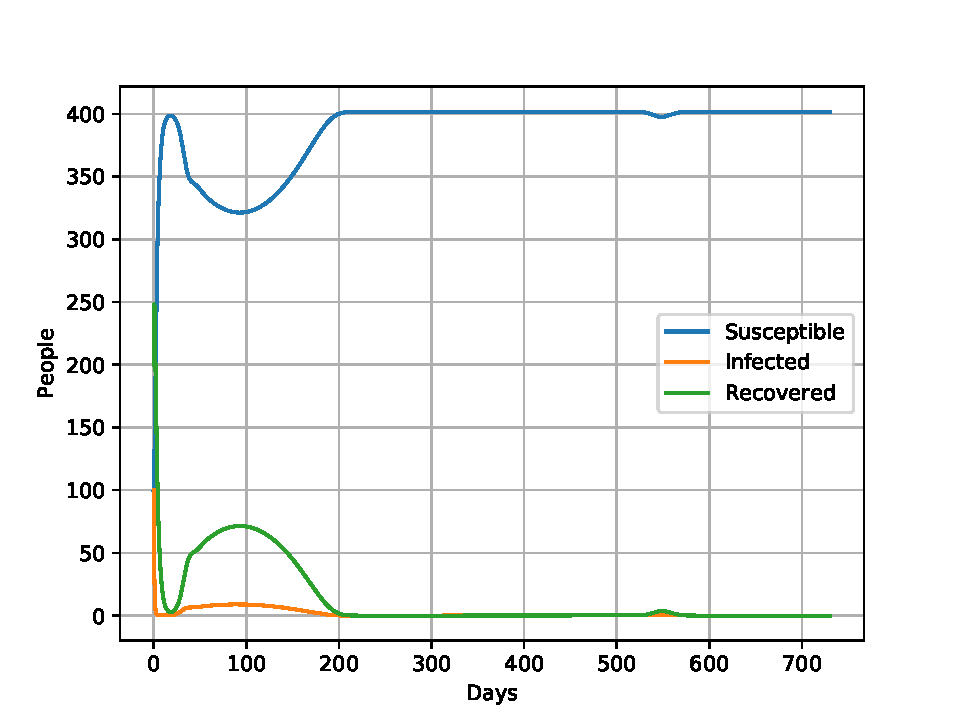
\includegraphics[scale=0.56]{../plots/opp_d_B.pdf}
		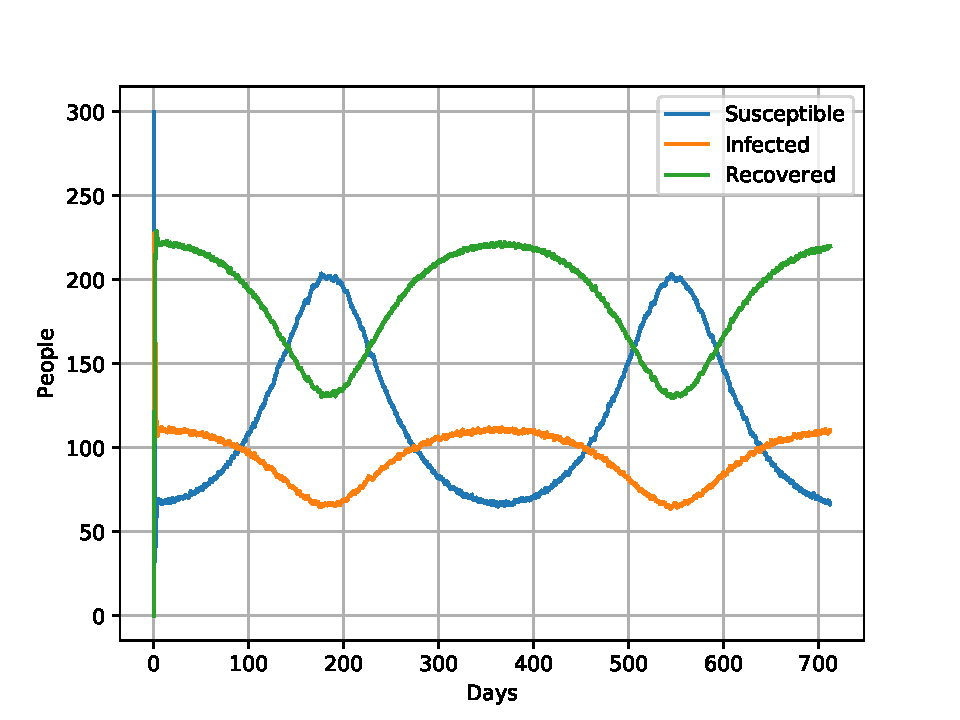
\includegraphics[scale=0.56]{../plots/opp_d_C_MC.pdf}
		\caption{Plots of populations when $a$ varies with time, found using Monte Carlo. Population $A$ on the left with $A=1$ and $a0=4$, and $B$ on the right with $A=2$ and $a0=4$.}
		%Label gjør det enkelt å referere til ulike bilder.
		\label{opp_d0_MC}
	\end{figure}
	
	
	\subsubsection{Vaccination}
	
	In figure \ref{opp_e0} you can see a plot of population $B$ with constant vaccination. 
	In figure \ref{opp_e1} you can see a plot of population $B$ with linear vaccination. 
	In figure \ref{opp_e2} you can see a plot of population $B$ with a vaccination campaign. 
	
	\begin{figure}[!htb]
		\centering 
		%Scale angir størrelsen på bildet. Bildefilen må ligge i samme mappe som tex-filen. 
		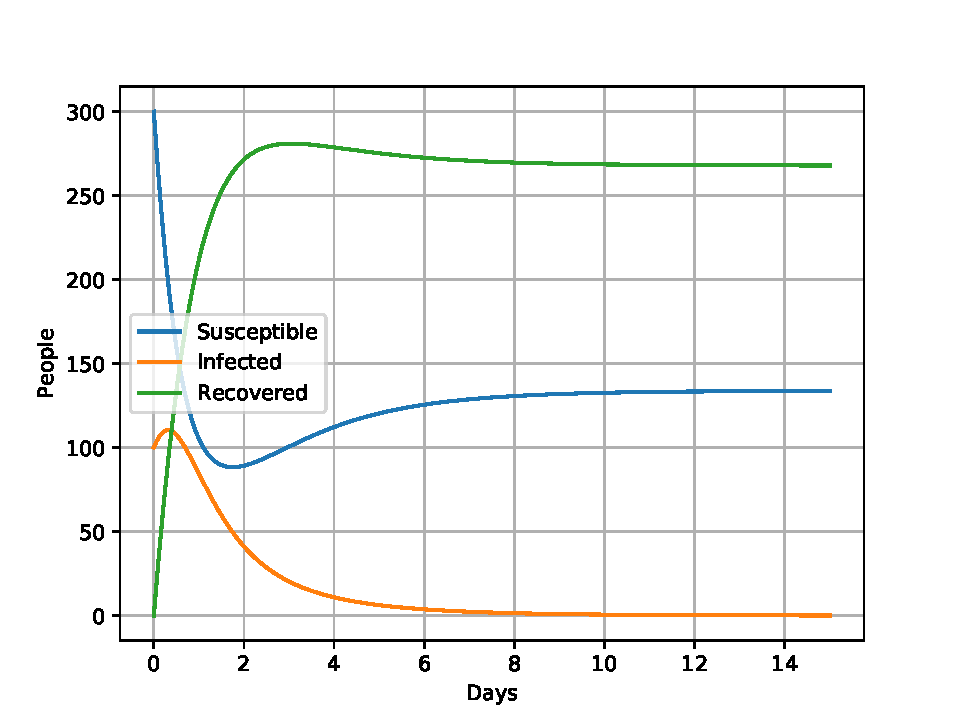
\includegraphics[scale=0.56]{../plots/opp_e_B0.pdf}	
		\caption{Plots of population $B$, found using Runge Kutta, with constant vaccination $f=1$.}
		%Label gjør det enkelt å referere til ulike bilder.
		\label{opp_e0}
	\end{figure}

	\begin{figure}[!htb]
		\centering 
		%Scale angir størrelsen på bildet. Bildefilen må ligge i samme mappe som tex-filen. 
		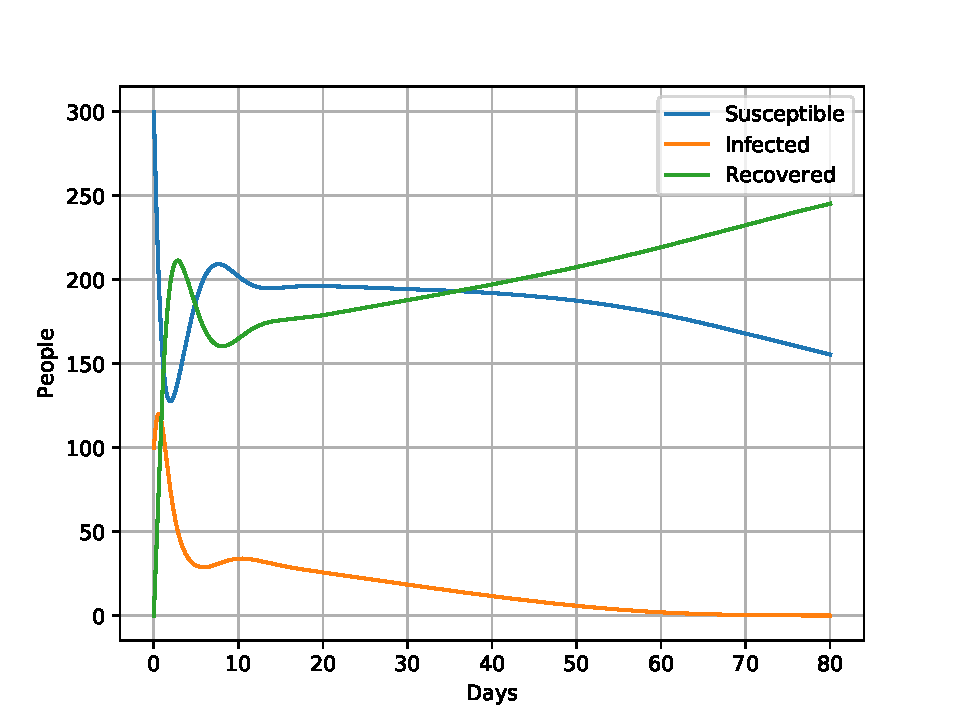
\includegraphics[scale=0.56]{../plots/opp_e_B2.pdf}	
		\caption{Plots of population $B$, found using Runge Kutta, with linear vaccination $f=0.1 t$.}
		%Label gjør det enkelt å referere til ulike bilder.
		\label{opp_e1}
	\end{figure}	

	\begin{figure}[!htb]
		\centering 
		%Scale angir størrelsen på bildet. Bildefilen må ligge i samme mappe som tex-filen. 
		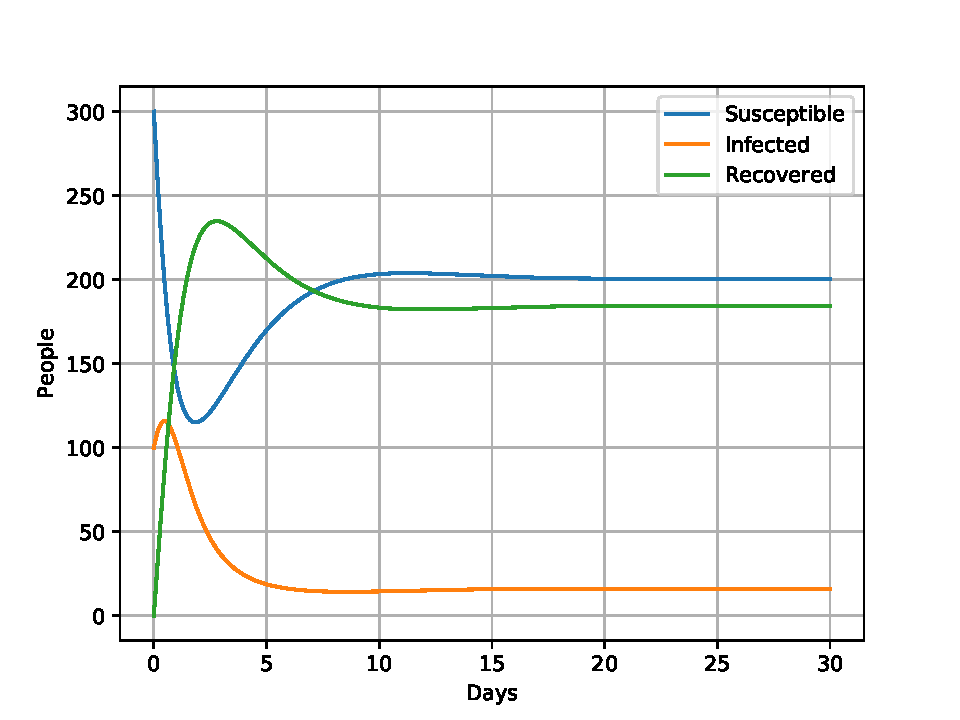
\includegraphics[scale=0.56]{../plots/opp_e_fb.pdf}	
		\caption{Plots of population $B$, found using Runge Kutta, with a vaccination campaign from day 2 to 9, where $f=0.3$, while it's 0 the rest of the time.}
		%Label gjør det enkelt å referere til ulike bilder.
		\label{opp_e2}
	\end{figure}

	In figure \ref{opp_e0_MC} you can see a plot of population $B$ with constant vaccination. 
	In figure \ref{opp_e1_MC} you can see a plot of population $B$ with linear vaccination. 
	In figure \ref{opp_e2_MC} you can see a plot of population $B$ with a vaccination campaign. 
	
	\begin{figure}[!htb]
		\centering 
		%Scale angir størrelsen på bildet. Bildefilen må ligge i samme mappe som tex-filen. 
		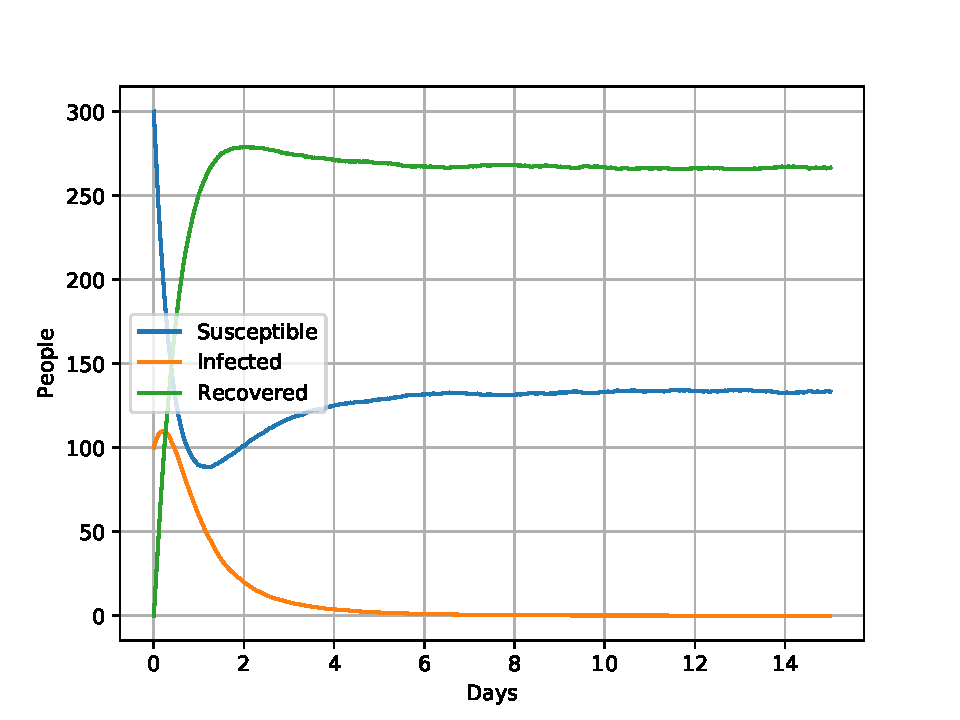
\includegraphics[scale=0.56]{../plots/opp_e_B0_MC.pdf}	
		\caption{Plots of population $B$, found using Monte Carlo, with constant vaccination $f=1$.}
		%Label gjør det enkelt å referere til ulike bilder.
		\label{opp_e0_MC}
	\end{figure}
	
	\begin{figure}[!htb]
		\centering 
		%Scale angir størrelsen på bildet. Bildefilen må ligge i samme mappe som tex-filen. 
		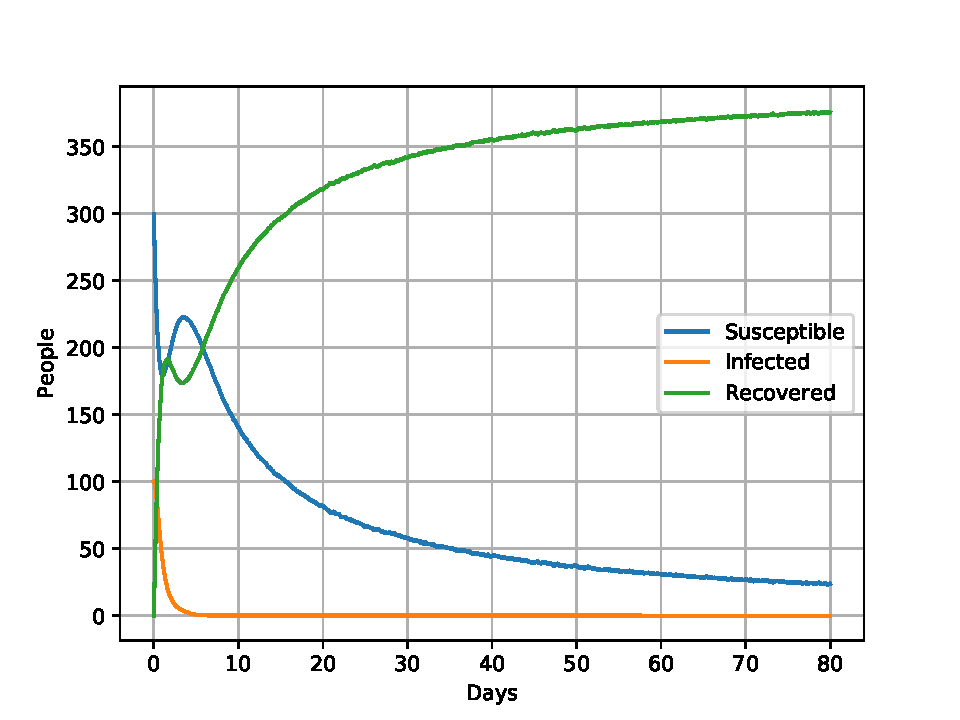
\includegraphics[scale=0.56]{../plots/opp_e_B2_MC.pdf}	
		\caption{Plots of population $B$, found using Monte Carlo, with linear vaccination $f=0.1 t$.}
		%Label gjør det enkelt å referere til ulike bilder.
		\label{opp_e1_MC}
	\end{figure}
	
	\begin{figure}[!htb]
		\centering 
		%Scale angir størrelsen på bildet. Bildefilen må ligge i samme mappe som tex-filen. 
		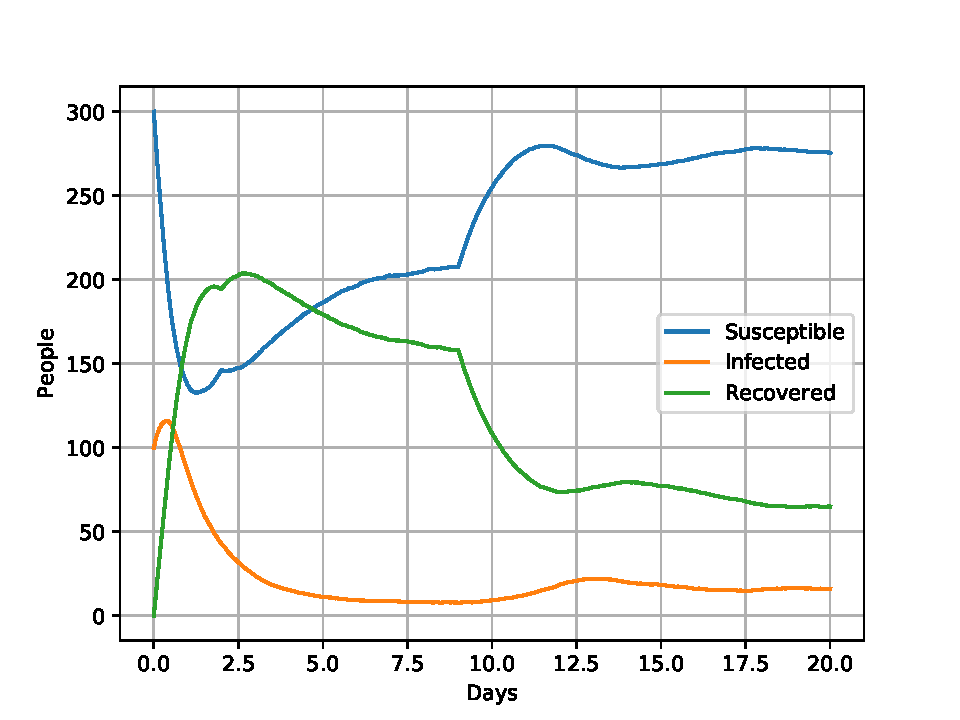
\includegraphics[scale=0.56]{../plots/opp_e_fb_MC.pdf}	
		\caption{Plots of population $B$, found using Monte Carlo, with a vaccination campaign from day 2 to 9, where $f=0.3$, while it's 0 the rest of the time.}
		%Label gjør det enkelt å referere til ulike bilder.
		\label{opp_e2_MC}
	\end{figure}

	\subsection{EFFICIENCY}
	Simulating with and without multithreading the only variables really effecting run time are number of timesteps $\frac{T}{\Delta t}$ and total simulations $sims$.
	\begin{table}[!htb]
		\centering
		\begin{tabular}{|l|l|l|}
			\hline
			Values & Seconds without multithreading & Seconds with multithreading \\ \hline
			$sims$ = 1000, $\frac{T}{\Delta t}=\frac{5\cdot 365.25}{0.0025}$ & 110.24 & 66.54 \\ \hline
		\end{tabular}
	\end{table}
	Based on several runs these values are representative for the average values.
	\section{DISCUSSION}
	\subsection{Runge Kutta against Monte Carlo}
	\subsubsection{The SIRS model and Runge Kutta}
	From figure \ref{fig:opp_a_A} to \ref{fig:opp_a_D} and table \ref{tab:opp_a_A} to \ref{tab:opp_a_D} we can see that our Runge Kutta algorithm produces about the same values as the expected analytical values. This suggest that our model is a good approximation. We can also see that the number of people doesn't equal exact integers, but rather a decimal number. This is expected as Runge Kutta is only a numerical approximation and is indiscreet. What is not expected is that the total population increases with about 1 to 2 people. This is likely due to numerical errors, but since this constitutes less than $1\%$ of the population it is probably safe to ignore this. A smaller $\Delta t$ would probably make this error smaller. 
	
	From figure \ref{fig:opp_a_E} and table \ref{tab:opp_a_E} we can see that the plot for population $E$ and $D$ is about the same, with the amount of infected decreasing faster for population $E$. The numerical end values are also about the same as for population $D$, however the expected values are outside the acceptable values for $s^*$, $i^*$ and $r^*$. 
	
	On figure \ref{opp_c0B} we can see that the values we chose for death and birth rate are too low to have a noticeable effect. If we ran the simulation for several years there might be an noticeable effect. From the plot on the right we can see that a value of $d_i = 0.1$ is quite significant and leads to steady decrease of the population. 
	
	From figure \ref{opp_c0} we can see that when $d_i=0.01$ the total population decreases quite slowly, with over half the population left after almost a year. It is unrealistic to assume that, when faced with such a decease, people wouldn't take more drastic measures to prevent the decease from spreading. We can also see that when $d_i=3$, all the infected people die within a couple of days, yet the total population decreases slowly after that. This is likely due to the fact that the amount of infected is not exactly zero, but close to it. This causes some people to become infected, and then immediately dying. If the simulation took account for this, all the infected people would die, and then the total population would remain constant. 
	
	In figure \ref{opp_c1} we can see a plot where the entire population dies within a year. In this case $d_i=0.1$, and it is more reasonable to assume that people wouldn't be able to take more drastic measures here, than for $d_i=0.01$, as people die at a much faster rate. 
	%After 100 days more than $\frac{3}{4}$ of the population is dead, and it's difficult for a community of people to do significant things when many of them are dead. (eller noe)
	In this plot the amount of infected, susceptible and recovered people reach zero at about the same time, meaning we don't have the same situation as for $d_i=3$, where people become infected even though there aren't any more infected people left. So if you are a bio-terrorist you should aim to create a disease with parameter similar to this one. 
	
	In figure \ref{opp_c2} you can see a population with an extreme population growth. This is of course high unrealistic, but is made to illustrate a population increasing over time. 
	
	In figure \ref{opp_d0} on the left, you can see a stable system where the amount of people in each group oscillates. However the amount of oscillation is quite low, with the amount of infected people not chaining with more than about $10-15$ people. Most disease that oscillates like this would probably have a higher amplitude. On the right you can see a plot with a higher amplitude, however this one has the problem of reaching zero infected people. At about day 300 the disease should have died out, yet it remains due to the limitations of Runge Kutta. The other curves also appear discontinuous at the points where infected people reach about zero.
	
	In figure \ref{opp_e0} it appears as if the disease dies out after about 8 days. A this point the vaccination would probably stop, but other than that this seems like a realistic plot. In figure \ref{opp_e1} the vaccination also manages to kill of the disease, but at slower rate. After this the amount of susceptible people goes to zero, while the amount of recovered goes towards 400. Again, the vaccination would probably stop here, but other than that this seems like a reasonable plot. In figure \ref{opp_e2} the vaccination campaign was not strong enough to kill of the disease, however it did make it so that the permanent infected population would be at a lower point than if it hadn't been done. So the campaign was a partial success.
	\subsubsection{Monte Carlo}
	For the discussion of the Monte Carlo simulations we will point to the key differences between the Runge Kutta method and the Monte Carlo method. 
	
	The first noticeable difference can be found by comparing figure \ref{opp_c0} and \ref{opp_c0_MC}. There is a clear tendency for the Runge Kutta simulation to have a decreasing population. On the other hand the Monte Carlo simulation gives a steady population. This could be because $I$ never truly becomes zero for the Runge Kutta simulation, and so someone will inevitably die. The Monte Carlo method, on the other hand has $I = 0$ from about day 5.
	
	Another big difference can be found between figure \ref{opp_c1} and \ref{opp_c1_MC}. For some reason the population doesn't die completely with a Monte Carlo simulation. We do not know why.
	
	Figure \ref{opp_c2} and \ref{opp_c2_MC} displays a major problem with the Monte Carlo simulation. In \ref{opp_c2_MC} the population stabilises at about 2000, because $\Delta t$ is too large.
	
	Finally we have figures \ref{opp_e0} through \ref{opp_e2_MC} , which are widely dissimilar. This is probably due to a bug in the implementation, rather than an inherent problem with one of the methods. We can however say from figure \ref{opp_e2_MC} that vaccination campaigns work.
	
	\subsection{EFFICIENCY}
	We would expect the efficiency increase from multithreading to be about $\frac{1}{3.5}$ the original time. We are running this program on computers with 4 cores and no hyper threading. Subtracting some efficiency for the multithreading overhead and the slightly lower CPU clock speeds at all-core full load we get about $\frac{1}{3.5}$. Our data didn't quite match up to expectations here. We saved about $40\%$ of our run time, which is a significant saving, but we were nowhere near the expected results.
	
	\section{CONCLUSION}
	%kan kaskje legges inn i discussion
	
	The Runge Kutta method is a good approximation to use on the SIRS method, but it has certain limitations, especially when the amount of infected people is close to zero. 
	
	The Monte Carlo method also has its limitations when we encounter low levels of infected people. Whenever $I$ is too low, there will be some simulations in which the population actually reaches zero, which means that the disease is eradicated, and any further increase in transmission rates has no effect. What this means is that we get extremely high standard deviations in the distribution of simulations that at any point gets close to zero infected. This doesn't mean that we get bad results, but rather that the average itself cant tell us as much.
	
	Another limitation is large populations. In our implementation $\Delta t$ is highly dependant on population size, and with a population the size of a country's we would get a $\Delta t$ so small that the simulation would last for ages, and we would need stupendous amounts of memory. 
	
	%\newpage
	\section{APPENDICES}
	All the calculations were done using the programming language Julia. The programs used can be found at:
	\url{https://github.com/UlrikSeip/Projects/tree/master/prosjekt5}.
	
	%\section{REFERENCES}
	\begin{thebibliography}{9}
		\bibitem{lecture notes}
		Computational Physics, Lecture Notes Fall 2015, Morten Hjort-Jensen p. 419-424
		\bibitem{wiki-d.rate}
		\url{https://en.wikipedia.org/wiki/List_of_sovereign_states_and_dependent_territories_by_mortality_rate}
		\bibitem{ssb-f.rate}
		\url{https://www.ssb.no/fodte/}
		\bibitem{wb-bef}
		\url{https://data.worldbank.org/indicator/SP.POP.TOTL?end=2017&start=2015&year_high_desc=true}
	\end{thebibliography}
	
	
	
	
	%\begin{figure}[h!]
	%	\centering 
	%	%Scale angir størrelsen på bildet. Bildefilen må ligge i samme mappe som tex-filen. 
	%	\includegraphics[scale=0.7]{opp2_7.pdf}
	%	\caption{A plot of the entropy}
	%	%Label gjør det enkelt å referere til ulike bilder.
	%	\label{2.7}
	%\end{figure}
	
	
	
	
	
	
	
	
	
	
	
	
	
	
	
	
	
	
	
	
	
	
\end{document}




